\documentclass[11pt,a4paper]{article}

% ----------------------------------------------------------------------
%  Cardiac shear-wave elastography processing — project summary
% ----------------------------------------------------------------------
\usepackage[utf8]{inputenc}
\usepackage[T1]{fontenc}
\usepackage{lmodern}
\usepackage[margin=2.4cm]{geometry}
\usepackage{graphicx}
\usepackage{booktabs}
\usepackage{amsmath}
\usepackage{siunitx}
\usepackage{xcolor}
\usepackage{caption}
\usepackage{subcaption}
\usepackage{enumitem}
\usepackage{microtype}
\usepackage[hidelinks,colorlinks=true,linkcolor=blue!55!black,citecolor=blue!55!black,urlcolor=blue!55!black]{hyperref}

\graphicspath{{figures/}}
\captionsetup{font=small,labelfont=bf}
\setlist{itemsep=2pt,topsep=3pt}

% Convenience boxes for "the good" and "caveat"
\newcommand{\good}[1]{\textcolor{green!45!black}{\textbf{#1}}}
\newcommand{\caveat}[1]{\textcolor{orange!75!black}{\textbf{#1}}}

\title{\vspace{-1.5em}\textbf{Cardiac Shear-Wave Elastography: A Processing Pipeline,\\
Interactive Method-Exploration GUI, and What the Data Can and Cannot Give}\\[0.3em]
\large A summary of the \texttt{shearWaveProcessing} project}
\author{TU Eindhoven --- Shear-wave elastography}
\date{August 2026}

\begin{document}
\maketitle

\begin{abstract}
\noindent
This report summarises the work carried out in the \texttt{shearWaveProcessing} repository, a unified
pipeline for cardiac shear-wave elastography (SWE) that takes raw Verasonics RF through beamforming to
the shear-wave \emph{space-time} plots from which propagation speed (and hence stiffness) is read. The
project spans three very different data sources --- a calibrated CIRS phantom, the published Caenen
\emph{et al.} pig ARF-SWE dataset, and our own transthoracic in-vivo human recordings --- and combines a
modular processing pipeline, an interactive method-exploration GUI, and a substantial human-in-the-loop
scoring campaign to decide which processing choices matter and which metrics reflect image quality.
The headline results are positive and, we believe, honest: on the phantom we established a clean,
voltage-monotonic ARF wave and a settled, \emph{SNR-adaptive} recipe; on the Caenen pig data we recover
a clean symmetric shear wave at every push, validating that the pipeline works on a \emph{real} cardiac
ARF wave. The one clear negative --- and it is a clear one --- is that our current in-vivo human
acquisition does \emph{not} contain a recoverable ARF wave: it is dominated by cardiac wall motion and is
\emph{acquisition-limited} (an underpowered, deep, loose-focus push), not primarily processing-limited.
The report closes with a concrete, evidence-backed set of acquisition changes (a stronger push via a
larger aperture and a longer pulse) that should close this gap.
\end{abstract}

% ======================================================================
\section{Introduction and scope}
% ======================================================================
Shear-wave elastography estimates tissue stiffness from the propagation speed of a shear wave. In the
heart this is done in two ways: \textbf{active} SWE induces a wave with a focused acoustic-radiation-force
(ARF) ``push'' and tracks it at a high frame rate, and \textbf{passive} SWE reads the natural mechanical
waves launched by valve closure. Both are hard transthoracically: the small phased-array footprint limits
how strong a push can be formed, the wall is deep, and the wall itself moves by tens of microns during the
cardiac cycle --- comparable to or larger than the wave we want to see \cite{strachinaru2020,vos2024}.

The pipeline reconstructs, per measurement, a \emph{space-time} image: displacement (or its temporal
derivatives) sampled along an anatomical ``M-line'' through the wall, as a function of distance along the
line ($r$) and slow time ($t$). A propagating wave appears as a tilted band whose slope is $1/c$; for a
symmetric ARF push about a focal point it forms a characteristic outward ``$\wedge$/V''. Everything in this
project is ultimately judged on whether that structure is present, clean, and consistent.

This document is organised around the deliverables requested: the data sources
(\S\ref{sec:data}), M-line selection and its variance (\S\ref{sec:mline}), the processing pipeline and its
method choices (\S\ref{sec:pipeline}), the exploration GUI (\S\ref{sec:gui}), the scoring experiments and
what metric survived them (\S\ref{sec:scoring}), the optimal phantom recipe and the voltage sweep
(\S\ref{sec:phantom}), acquisition-parameter recommendations (\S\ref{sec:acq}), the Caenen pig success
(\S\ref{sec:caenen}), the in-vivo failure (\S\ref{sec:invivo}), and next steps (\S\ref{sec:next}).

% ======================================================================
\section{Data sources}\label{sec:data}
% ======================================================================
Three data sources drive the project, spanning ``easy and controlled'' to ``hard and realistic''
(Table~\ref{tab:data}).

\begin{description}[leftmargin=1.2em]
  \item[Phantom (CIRS).] A static, homogeneous calibrated phantom imaged with our own S5-1 sequence. Because
  it is static there is \emph{no} cardiac motion, so it is the clean reference case. Two campaigns were
  acquired: an 8-level \textbf{transmit-voltage sweep} (15--50\,V, the SNR knob) and an 11-configuration
  \textbf{acquisition-parameter sweep} (push pulse length, aperture, and tracking PRF). The push produces a
  wave that is symmetric about the focus, so the M-line is a horizontal line at the focal depth --- no
  interactive drawing needed.
  \item[Caenen pig ARF-SWE.] The published dataset from Caenen \emph{et al.}, \emph{Sci.\ Rep.}\ 2023
  \cite{caenen2023}: transthoracic PLAX pig hearts, R-peak-triggered, 52 pushes per cardiac cycle. This is a
  \emph{real cardiac ARF wave} acquired with a much stronger, shallower, tightly-focused push (F/1 at
  25\,mm) --- the ideal external validation that our pipeline works on cardiac data. Ingested through a
  cropped Cartesian bridge (\texttt{swp\_gui/caenen.py}).
  \item[In-vivo human (our acquisition).] Transthoracic PLAX septum (subject ``Luuk''), S5-1 phased array,
  free-running, 24 ARF pushes over a cardiac cycle, at 30\,V and 40\,V. This is the target application and,
  as \S\ref{sec:invivo} shows, the hardest case.
\end{description}

\begin{table}[t]
\centering\small
\caption{The three data sources and the key acquisition parameters that separate them. The in-vivo/Caenen
gap (push F-number, focal depth, tracking PRF, cardiac gating) is the crux of \S\ref{sec:invivo}.}
\label{tab:data}
\begin{tabular}{@{}lccc@{}}
\toprule
 & \textbf{Phantom (ours)} & \textbf{In-vivo human (ours)} & \textbf{Caenen pig} \\
\midrule
Subject / view        & CIRS phantom          & Human PLAX septum        & Pig PLAX septum \\
Probe                 & S5-1 (80 el.)         & S5-1 (80 el.)            & P4-2 (128 el.) \\
Push F-number         & 8.4--2.5 (swept)      & $\approx 4.3$            & \textbf{1} \\
Push focal depth      & 49\,mm                & 44.6\,mm                & 25\,mm \\
Push voltage          & 15--50\,V (swept)     & 30 / 40\,V              & 50--60\,V (MI 2.2) \\
Push duration         & 448--851\,\si{\micro s} & 667\,\si{\micro s}    & 800\,\si{\micro s} \\
Tracking PRF          & 3.7\,kHz              & 3.7\,kHz                & \textbf{8.8\,kHz} \\
Cardiac sync          & n/a (static)          & \textbf{free-running}   & \textbf{R-peak triggered} \\
Wall motion           & none                  & 20--40\,\si{\micro m}   & present, gated \\
\bottomrule
\end{tabular}
\end{table}

% ======================================================================
\section{M-line selection and its variance}\label{sec:mline}
% ======================================================================
The space-time plot is sampled along an \textbf{M-line} through the myocardial wall. For in-vivo/pig data
this line is anatomical and is drawn \textbf{manually}: the operator clicks points on the co-registered
B-mode frame (buffer~5 for active pushes, the buffer-4 stream for passive windows), which are resampled
into a \textbf{constant-arc-length spline}. The line is saved (\texttt{output/mlines/*.npz}) and reused
automatically on later runs, so batch processing is unattended once the lines exist. To reduce noise, the
pipeline also samples several \emph{parallel offset copies} of the line (along its normal) and combines them
(mean or median) --- a cheap, wavefront-preserving denoiser tailored to the anatomy.

\paragraph{Variance --- an honest limitation.} Manual selection is a genuine source of variability, and we
treat it as such rather than hiding it:
\begin{itemize}
  \item \textbf{Between pushes.} For the 24 in-vivo pushes the M-line is drawn once \emph{per push} (the wall
  moves), so each space-time image carries its own line. This is the most faithful choice but means the line
  geometry is not identical across pushes, which contributes to push-to-push spread independent of physiology.
  \item \textbf{Absolute speed is M-line-alignment-limited.} The single biggest \emph{accuracy} caveat of the
  passive analysis is that the measured speed depends on how well the M-line follows the true propagation
  path; obliquity of the oblique septum relative to the line biases the apparent speed. Across passive windows
  the \emph{visual} conclusions (a wave is present, in a given direction) are robust, but the \emph{absolute}
  speed numbers are not, and MVC-vs-AVC ordering did not always match literature --- we attribute this to
  line obliquity, not to the estimator.
  \item \textbf{Mitigations in place.} The offset-line averaging above; index-keyed saved lines so a given
  window always reuses the same geometry; and, for the phantom, a purely geometric horizontal line (no manual
  step) so the phantom results carry \emph{zero} M-line variance --- which is one reason the phantom is the
  trustworthy anchor for the method study.
\end{itemize}
A curvature/obliquity check and (for vertical lines) origin-relative direction naming are noted as
improvements (\S\ref{sec:next}).

% ======================================================================
\section{Processing pipeline}\label{sec:pipeline}
% ======================================================================
The pipeline is three modular stages driven by \texttt{run.py}, each runnable on its own if its inputs
exist:
\begin{enumerate}
  \item \textbf{convert} --- Verasonics \texttt{.mat} $\rightarrow$ zea \texttt{.hdf5} (RF buffers). If only
  the runtime parameter file is present, a merged \texttt{CombinedData.mat} is built first.
  \item \textbf{beamform} --- RF $\rightarrow$ complex IQ + B-mode, saved crucially \emph{with the ARF push
  location} (\texttt{custom/push\_focus\_x/z}) and all scan parameters, so downstream stages need only the IQ
  file. Storing the push location was a real gap we closed: the wave origin $r_0$ is now anchored on the
  \emph{stored} push, not a hard-coded guess.
  \item \textbf{viz} --- IQ $\rightarrow$ space-time plots ($+$ speed), for active (buffer~2) and passive
  (buffer~4) SWE, each with its own YAML recipe.
\end{enumerate}

The visualization core (stage 3) is a chain of interchangeable steps, each with a literature-backed rationale
(full review in \texttt{docs/literature\_review.md}). The steps, and the reasoning for the methods exposed at
each, are:

\begin{description}[leftmargin=1.2em]
  \item[1. IQ/RF pre-filter.] Optional slow-time/spatial low-pass (mild denoise), \emph{SVD clutter}
  filtering (removes the dominant low-rank bulk-tissue subspace --- the standard ultrafast-Doppler clutter
  filter \cite{demene2015}), and \emph{bulk-motion compensation} (undo the global per-frame translation on
  the IQ before tracking). \emph{Reasoning:} act on the raw signal before phase estimation, where clutter is
  best separated.
  \item[2. Displacement estimation.] \emph{Loupas} 2-D autocorrelation (phase-based, fast, as accurate as
  cross-correlation for small displacements \cite{pinton2006}) is the default; \emph{Kasai}, complex-IQ
  \emph{cross-correlation}, and \emph{RF cross-correlation on a locally re-beamformed fine axial grid} are
  alternatives. Choice of \emph{quantity} --- displacement / velocity / acceleration --- changes the
  estimate; acceleration is sharpest but noisiest \cite{petrescu2022}. An \emph{adaptive axial kernel} sizes
  the tracking window per pixel by local RF coherence. \emph{Reasoning:} Loupas is the community default and
  the upgrade Caenen themselves recommend over Kasai.
  \item[3. Cardiac-motion removal (the crux in vivo).] From assume-the-band to measure-the-motion: temporal
  band-pass / high-pass, polynomial detrend, SVD-on-displacement, \emph{reference} poly-extrapolation
  (fit motion on the pre-push frames, subtract), \emph{reference-subspace projection} (project out the SVD
  subspace of pre-push motion), phase-unwrap, and axial strain (invariant to uniform translation). Directional
  filtering (below) also rejects non-propagating bulk bands \cite{manduca2003}. \emph{Reasoning:} a fixed
  band-pass either passes bulk motion (low corner) or attenuates slow waves (high corner); reference-trained
  filters \emph{measure} the motion the fit never sees the wave.
  \item[4--5. Spatial \& temporal smoothing.] Gaussian, edge-preserving median, bilateral, non-local means,
  Perona--Malik and coherence-enhancing (tensor) diffusion; temporal moving mean/median and Savitzky--Golay.
  \emph{Reasoning:} suppress speckle noise while keeping the wavefront sharp (blurring it biases the speed).
  \item[6. M-line offset averaging] (\S\ref{sec:mline}).
  \item[7. Directional filter.] $(k,\omega)$ decomposition to keep outward / one-sided propagation and reject
  reflections, standing waves, and \emph{non-propagating uniform bulk bands}. This filter was found to be
  \good{decisive for active SWE (outward)} and was \emph{fixed} mid-project (a Tukey-windowed FFT with a
  smooth angular mask now nulls the opposite lobe by $\sim$80\%, versus $\sim$45\% before).
  \item[8. Speed + quality.] Time-of-flight$+$RANSAC, Radon / signed slant-stack (removes the per-time
  spatial mean to reject the flat bulk band \cite{mclaughlin2010}), plus quality metrics (\S\ref{sec:scoring}).
\end{description}

Both active and passive paths always emit \textbf{three independent recipes} (``views'') per measurement, so
a structure present in all three is more trustworthy than one that appears in a single tuning.

% ======================================================================
\section{The method-exploration GUI}\label{sec:gui}
% ======================================================================
A recurring difficulty is that ``which combination of steps is best'' is not obvious from theory and shifts
with SNR and data source. To make this tractable we built an interactive \textbf{Streamlit GUI}
(\texttt{swp\_gui/}) to experiment visually with every step from IQ/RF to the space-time plot.

Its design reflects hard-won lessons:
\begin{itemize}
  \item \textbf{Every stage is a live, ordered add/remove chain of methods}, each with tunable parameters and
  an \emph{inline source-code viewer}, so the operator sees exactly what each step does. Steps can be
  enabled/disabled and reordered.
  \item \textbf{Displacement, velocity and acceleration are shown together}, with a before/current/previous
  comparison grid so the effect of a change is immediately visible.
  \item \textbf{The acquisition constants are shown read-only} ($f_0$, demod frequency, PRF, $c$, $dz$) ---
  they come from the Verasonics data and must not be ``tuned''. This prevents a common error.
  \item \textbf{A built-in no-push control} runs the identical recipe on the pre-push reference window (where
  no push fired). This is the single most important diagnostic in the whole project (\S\ref{sec:invivo}): a
  recipe that produces a ``clean wave'' from the reference is imaging motion, not the push.
  \item Manual 2-click speed overlay, an SVD singular-value spectrum when tuning clutter cutoffs, a
  Caenen-data loader, and an ``animate all pushes'' export. It boots in $\sim$4\,s (heavy \texttt{zea}/torch
  imports are lazy).
\end{itemize}
New, reusable algorithms developed for the GUI live in \texttt{src/swp/viz/} and work through the batch
pipeline too, so nothing is GUI-only.

% ======================================================================
\section{Scoring experiments: which metric reflects quality?}\label{sec:scoring}
% ======================================================================
To decide \emph{objectively} which processing combinations are good --- and, more subtly, \emph{which scalar
metric agrees with a human looking at the plot} --- we ran a large blind human-in-the-loop scoring campaign.
Around 600 randomized and focused recipes were rendered as space-time plots across phantom 15/25/30/50\,V and
in-vivo 30/40\,V, and graded blind by the operator, both on an absolute 1--5 scale
(\texttt{score\_app.py}) and via 2-alternative forced-choice pairwise comparisons
(\texttt{pairwise\_app.py}, analysed with Bradley--Terry). Recipe features were then correlated with the
human scores (\texttt{metric\_experiment\_*.py}). The findings were genuinely instructive, including where
they were negative:

\begin{itemize}
  \item \caveat{A bespoke ``push-specificity'' metric was debunked.} We built a metric intended to reward a
  push-specific wave (push coherence discounted by no-push coherence). Blind grading showed it correlated
  \emph{worse} with humans than the simpler baseline it was meant to replace (Spearman $\rho\approx0.12$--0.17
  vs $\approx0.30$--0.37), with both false positives (noise scored high) and false negatives (clean smooth
  waves scored zero). It was retired.
  \item \good{\texttt{origin\_coherence} (averaged over quantities) is the metric to use.} It is the
  best-validated single scalar ($\rho\approx0.45$ across datasets, up to $0.60$ on clean phantom data), it
  \emph{generalises to in-vivo for ranking recipes}, and it has no blow-ups. It is now the $\star$ headline
  metric in the GUI (Fig.~\ref{fig:crossdataset}).
  \item \good{Human preference is legible.} Pooling 220 blind labels, the family the human rewards is clear:
  \emph{Loupas $+$ relative-to-reference $+$ temporal band-pass $+$ moderate smoothing $+$ moving-mean $+$
  OUTWARD directional $+$ several M-line offsets}. Frame-to-frame, IQ SVD/slow-time high-pass, bilateral,
  and one-sided directional filters consistently \emph{hurt}.
  \item \caveat{A ceiling of $\rho\approx0.5$ is honest.} Human scores are discrete and often near-ties, so a
  scalar cannot reproduce the exact ordering; the metric is good enough to \emph{rank} and \emph{flag}
  good-vs-bad, not to reproduce a fine ordering. Hand-crafted smoothness/symmetry additions did not robustly
  beat \texttt{origin\_coherence}.
\end{itemize}

\begin{figure}[t]
\centering
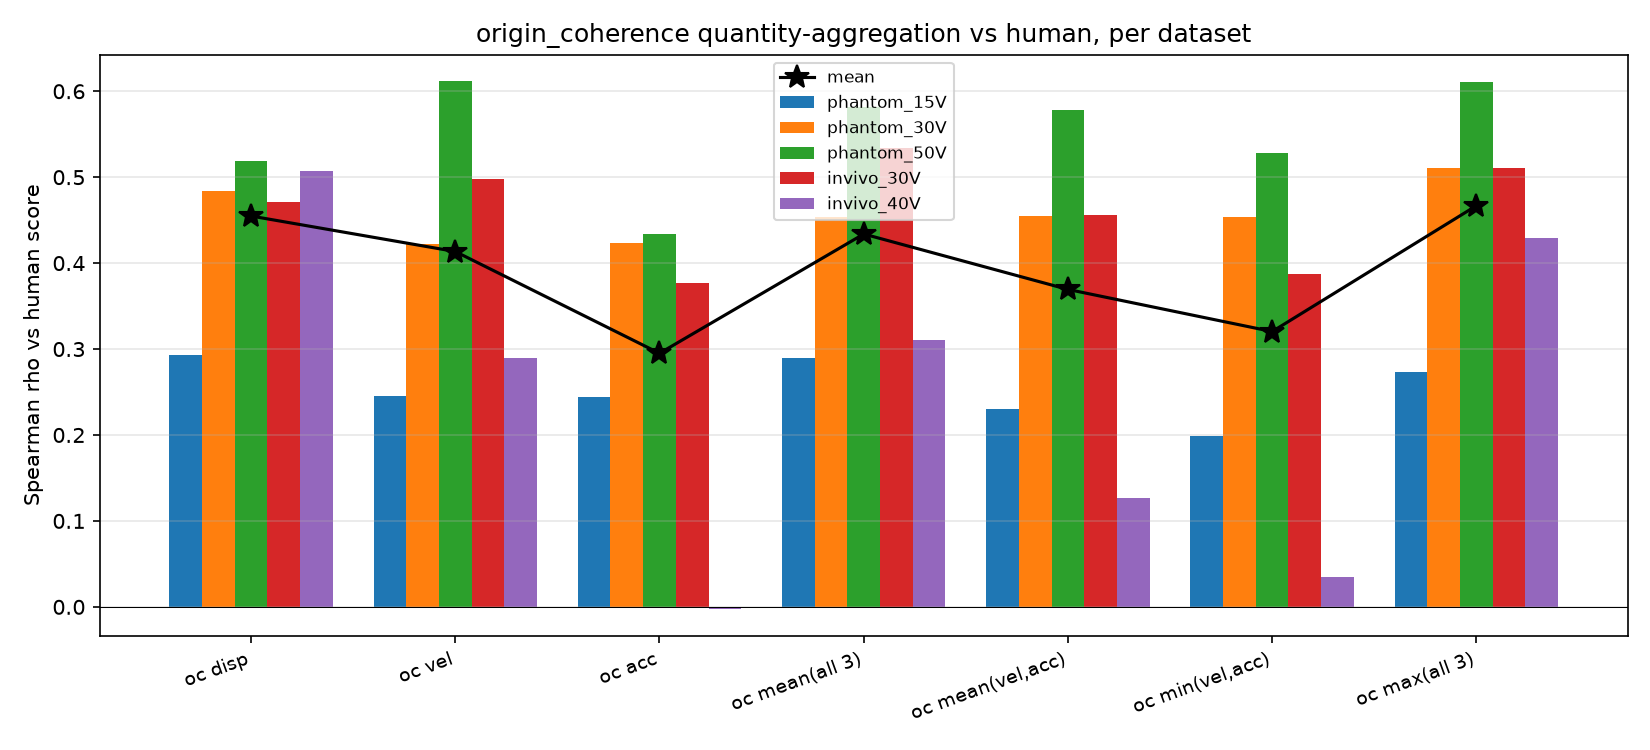
\includegraphics[width=0.86\textwidth]{crossdataset.png}
\caption{Cross-dataset metric validation. \texttt{origin\_coherence} generalises across phantom voltages and
in-vivo (Spearman $\rho\approx0.29$--0.61 vs blind human scores), does \emph{not} catastrophically break in
vivo for \emph{ranking} recipes, and has no false-positive/negative blow-ups --- which is why it, and not the
bespoke push-specificity metric, was adopted as the headline quality metric.}
\label{fig:crossdataset}
\end{figure}

A second, decisive lesson (Fig.~\ref{fig:snr}): \good{the optimal recipe is SNR-adaptive}. On phantom 30\,V
vs 50\,V pairwise grading, the readable \emph{quantity} shifts (high SNR $\rightarrow$
acceleration/velocity; low SNR $\rightarrow$ displacement; velocity is the most SNR-robust), and the optimal
\emph{smoothing} flips sign (light smoothing best at high SNR, heavier smoothing best at low SNR). A single
fixed recipe is therefore wrong; the recommendation is SNR-adaptive smoothing (tied to the Loupas
adaptive kernel) and a quantity that defaults to velocity or is chosen by SNR.

\begin{figure}[t]
\centering
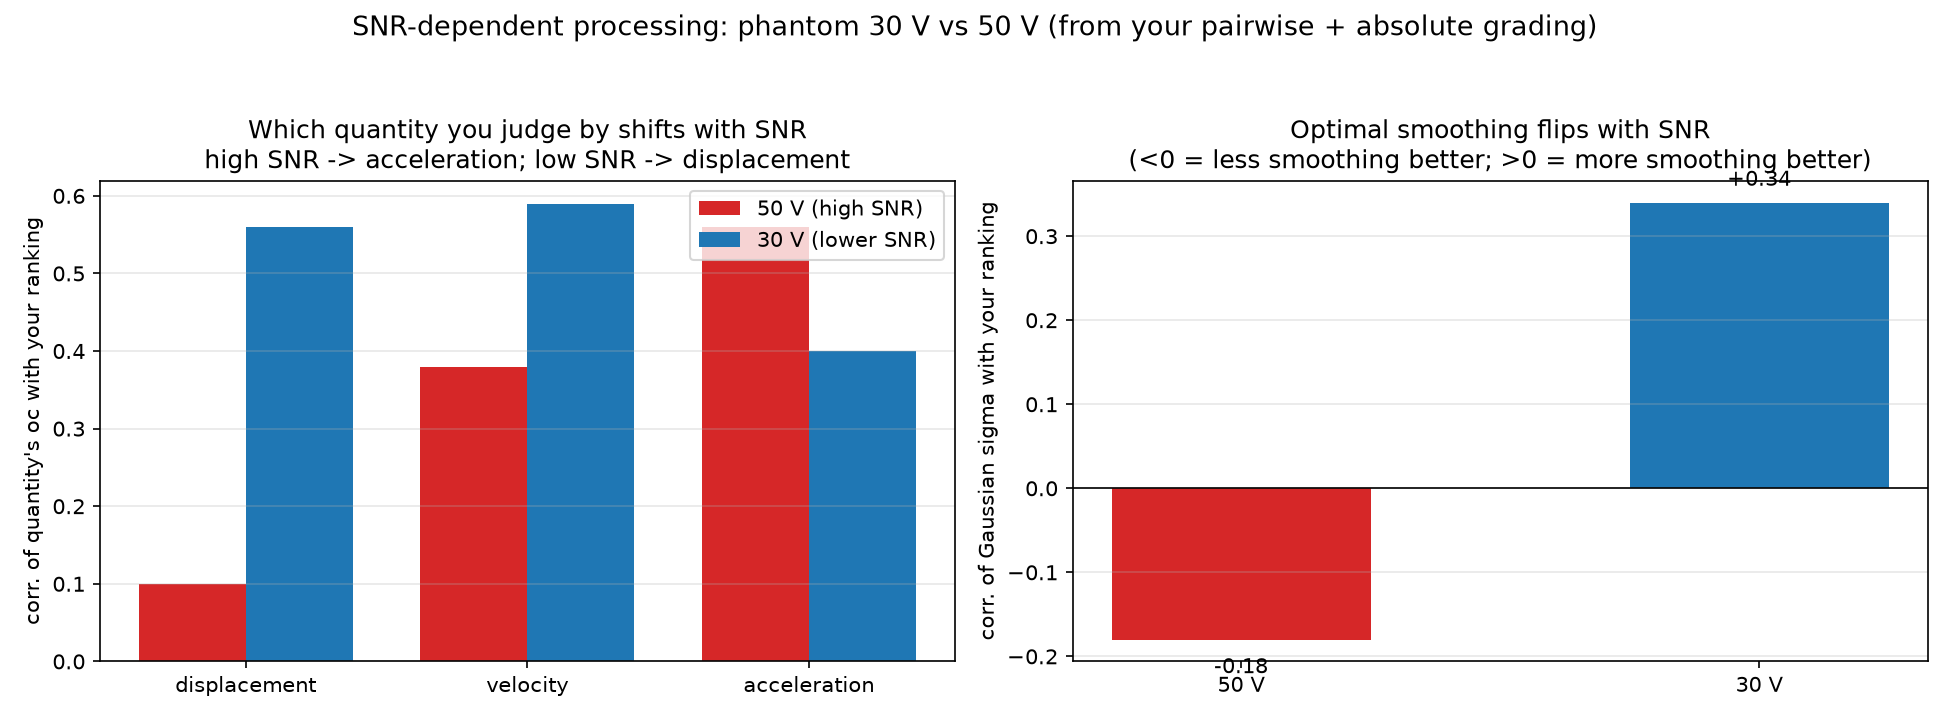
\includegraphics[width=0.92\textwidth]{snr_conclusion.png}
\caption{The settled recipe is \textbf{SNR-adaptive}, confirmed by blind pairwise grading. \emph{Left:} the
quantity that best matches human ranking shifts from acceleration (high SNR, 50\,V) to displacement (lower
SNR, 30\,V); velocity is robust to both. \emph{Right:} the correlation of Gaussian smoothing strength with
human ranking flips sign --- less smoothing is better at high SNR, more smoothing is better at low SNR.}
\label{fig:snr}
\end{figure}

% ======================================================================
\section{Optimal combination on phantom data}\label{sec:phantom}
% ======================================================================
The phantom is the clean anchor: static, no cardiac motion, and (for the voltage sweep) driven only by SNR.

\paragraph{Voltage sweep --- the reference result.} Figure~\ref{fig:voltage} is the requested space-time
$\times$ transmit-voltage figure. After an initial sweep was found to be silently \emph{clamped} by the
push transmit-power profile (a lesson: always verify the \emph{delivered} voltage, not the requested one),
the re-acquired sweep delivered eight distinct, monotonic levels 50\,V $\rightarrow$ 15\,V. \good{Shear-wave
clarity increases monotonically with voltage}: at $\geq40$\,V a crisp symmetric outward ``$\wedge$'' emerges
from $r_0$ (\texttt{origin\_coherence} 0.93--0.98); by 25--15\,V it is progressively buried in edge clutter
and noise. This clean, expected behaviour is what makes the phantom trustworthy as the method reference.

\begin{figure}[t]
\centering
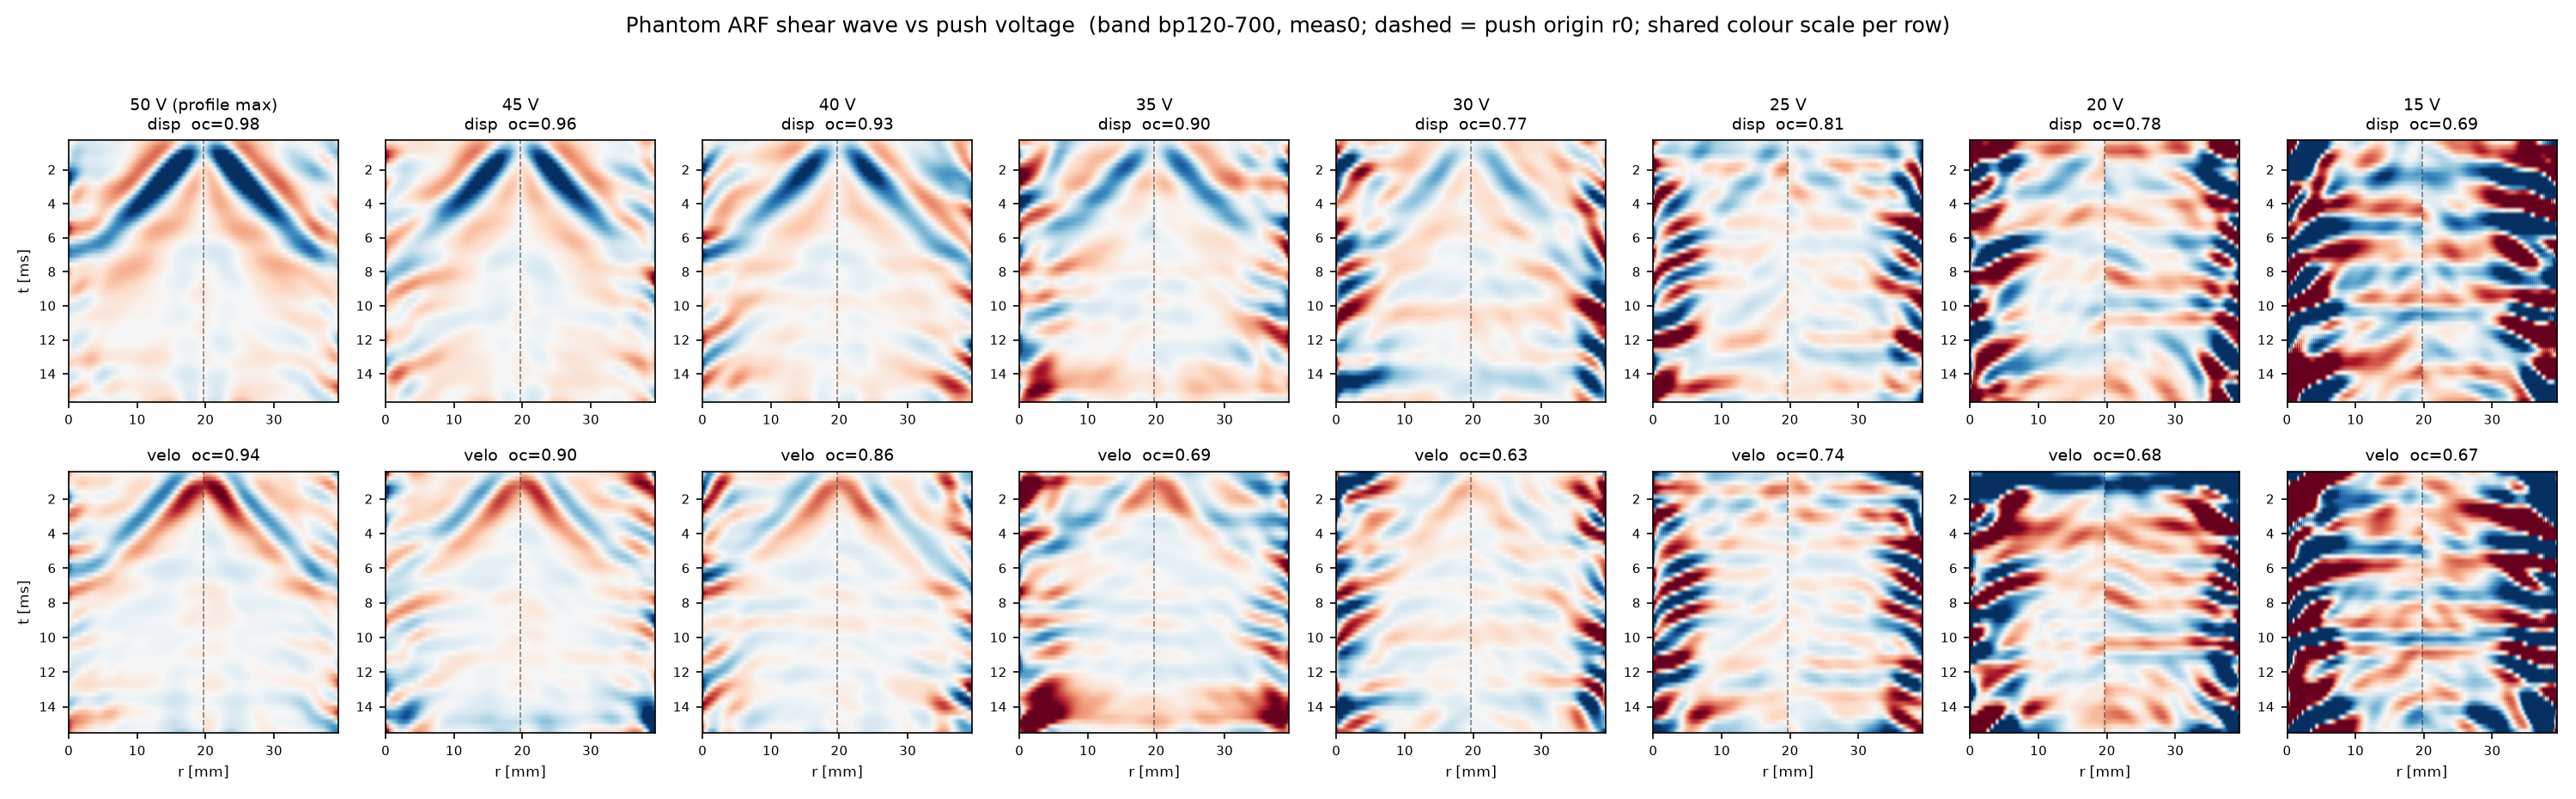
\includegraphics[width=\textwidth]{phantom_voltage_montage.png}
\caption{Phantom ARF shear-wave space-time as a function of push transmit voltage (50\,V $\rightarrow$
15\,V, left to right; top row displacement, bottom row velocity). The dashed line marks the push origin
$r_0$; colour scale is shared per row. Clarity is monotonic in voltage: a crisp symmetric outward wave at
$\geq40$\,V degrading smoothly into noise by 15\,V. \texttt{origin\_coherence} annotated per panel.}
\label{fig:voltage}
\end{figure}

\paragraph{The settled recipe.} From the scoring campaign and a dedicated low-SNR extraction sweep
(700 recipes $\times$ 8 voltages $\times$ 3 quantities $=$ 16\,800 evaluations), the settled family is:
\emph{Loupas $\cdot$ relative-to-reference $\cdot$ temporal band-pass $\cdot$ outward directional (decisive)
$\cdot$ moving-mean temporal $\cdot$ 7--9 M-line offsets}, with smoothing and quantity chosen by SNR
(\S\ref{sec:scoring}). Two robust presets emerged --- a ``sharp, high-SNR'' recipe (band 120--800\,Hz,
median smoothing, velocity) and an ``all-SNR robust'' recipe \texttt{id438} (band 80--500\,Hz $\rightarrow$
spatial median $\rightarrow$ temporal median $\rightarrow$ 9 offsets $\rightarrow$ outward).

\paragraph{Low-SNR extraction --- the honest hard case, and a positive result.} Using two speed-free
detectors (ROI-contrast on a locked 50\,V template, and left/right mirror-symmetry --- deliberately
\emph{not} relying on a fitted speed, which is unreliable at low SNR), \good{the shear-wave ``V'' is
detectable at every voltage down to 15\,V} (ROI-contrast $0.52\rightarrow0.19$, above the $0.05$ no-wave
floor throughout, Fig.~\ref{fig:lowsnr}). Low SNR is thus a processing problem, not a missing-signal
problem. The optimal levers shift exactly as the SNR study predicted: heavier, larger-$\sigma$ Gaussian
smoothing; a narrower low-frequency band ($f_\mathrm{hi}$ collapsing $\sim$800\,$\rightarrow$350\,Hz);
displacement rather than velocity; and SVD IQ clutter starting to help below 25\,V. One clear negative:
\caveat{the fine-grid RF cross-correlation estimator underperformed Loupas at every voltage}, with the gap
\emph{widening} as SNR dropped (it needs speckle SNR the low-voltage data lacks) --- so it is not worth
expanding for this task.

\begin{figure}[t]
\centering
\begin{subfigure}{0.545\textwidth}
  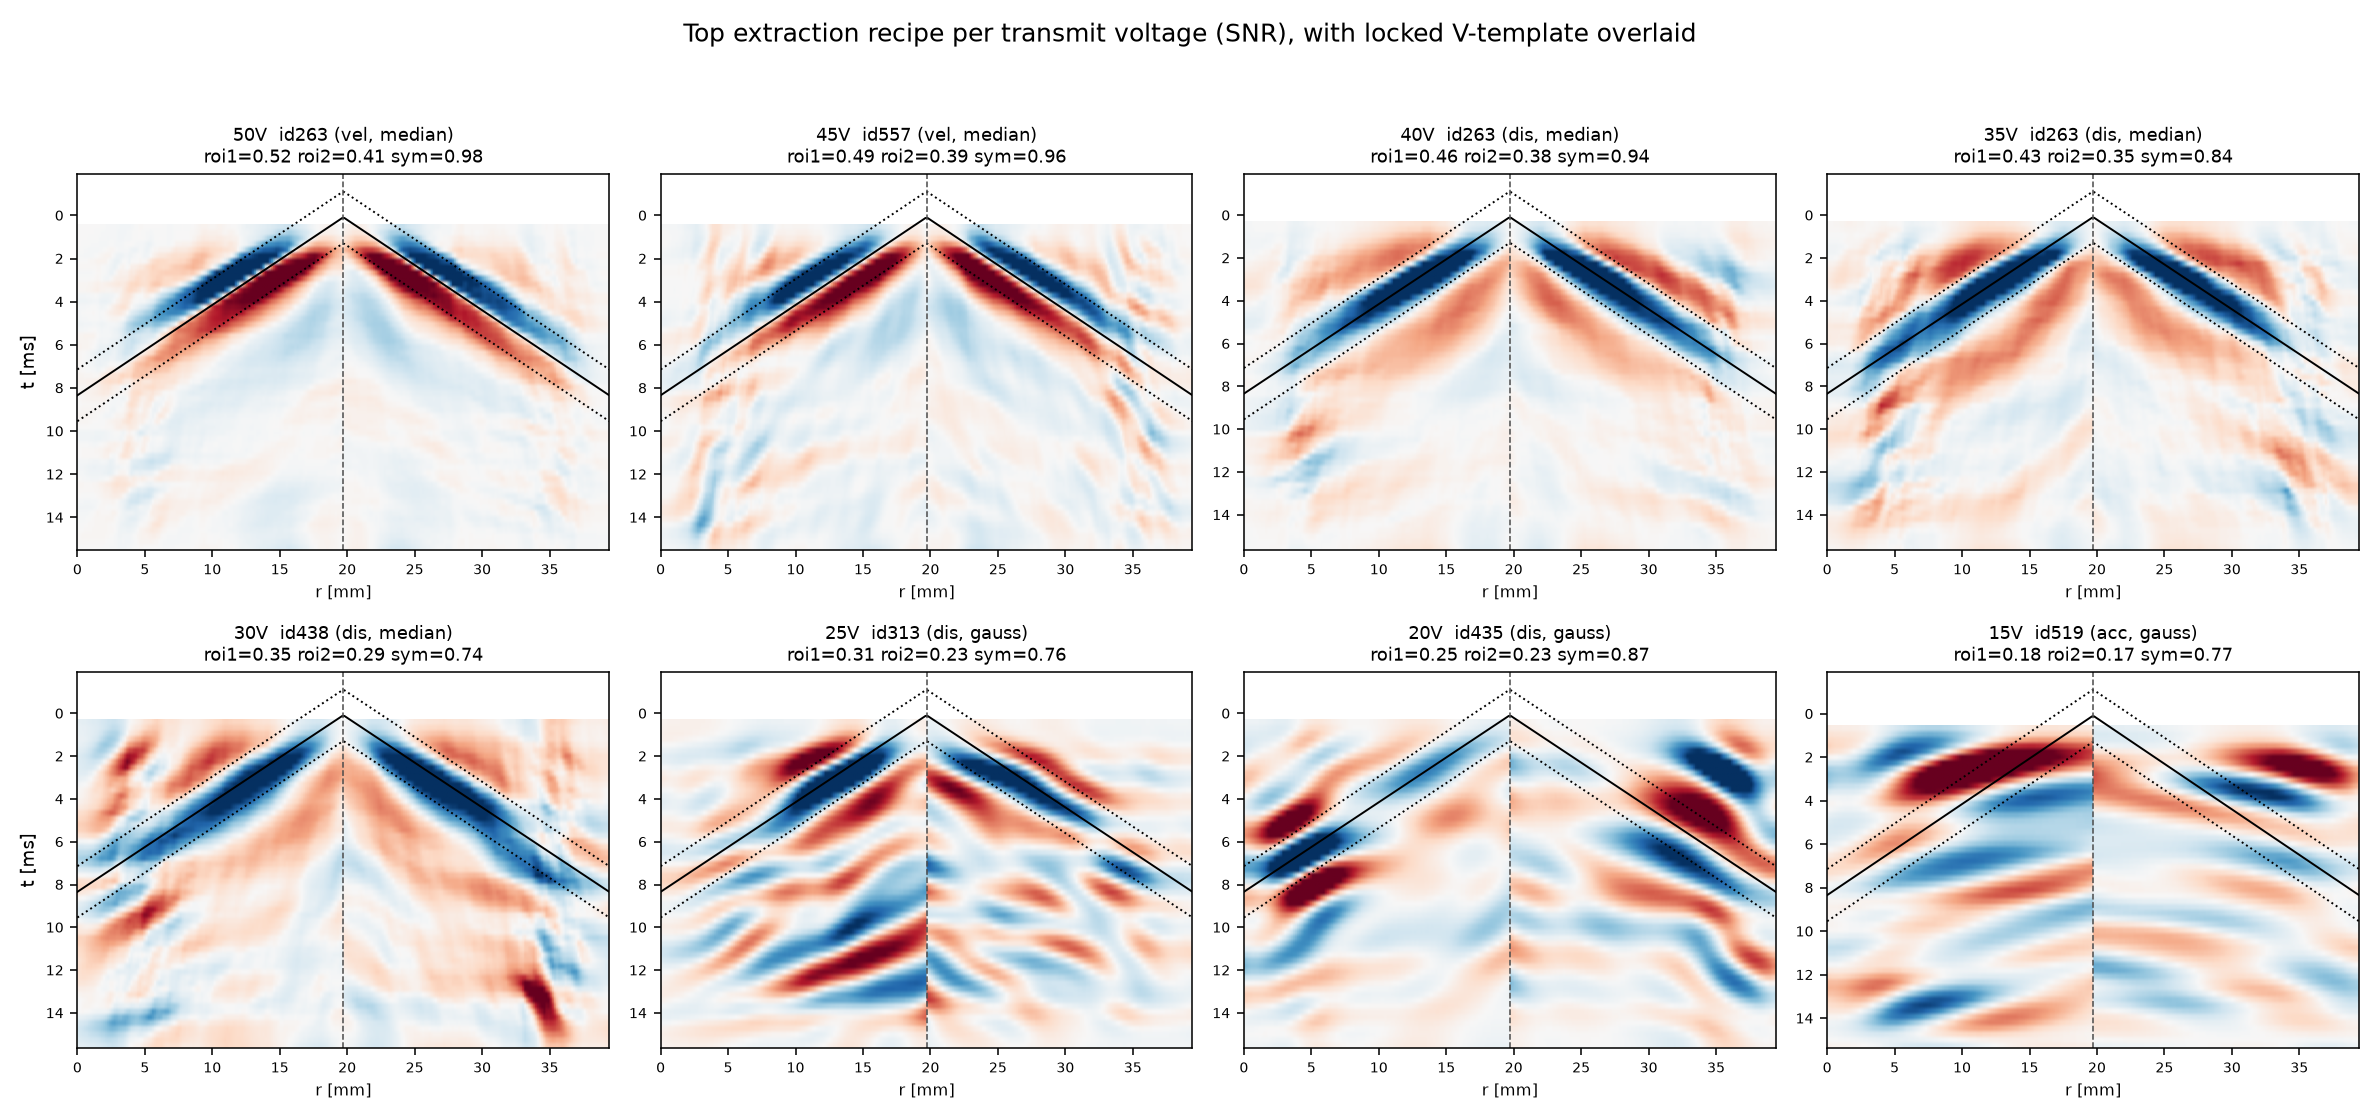
\includegraphics[width=\textwidth]{sweep_top_montage.png}
  \caption{Best recipe per voltage, V-template overlaid.}
\end{subfigure}\hfill
\begin{subfigure}{0.44\textwidth}
  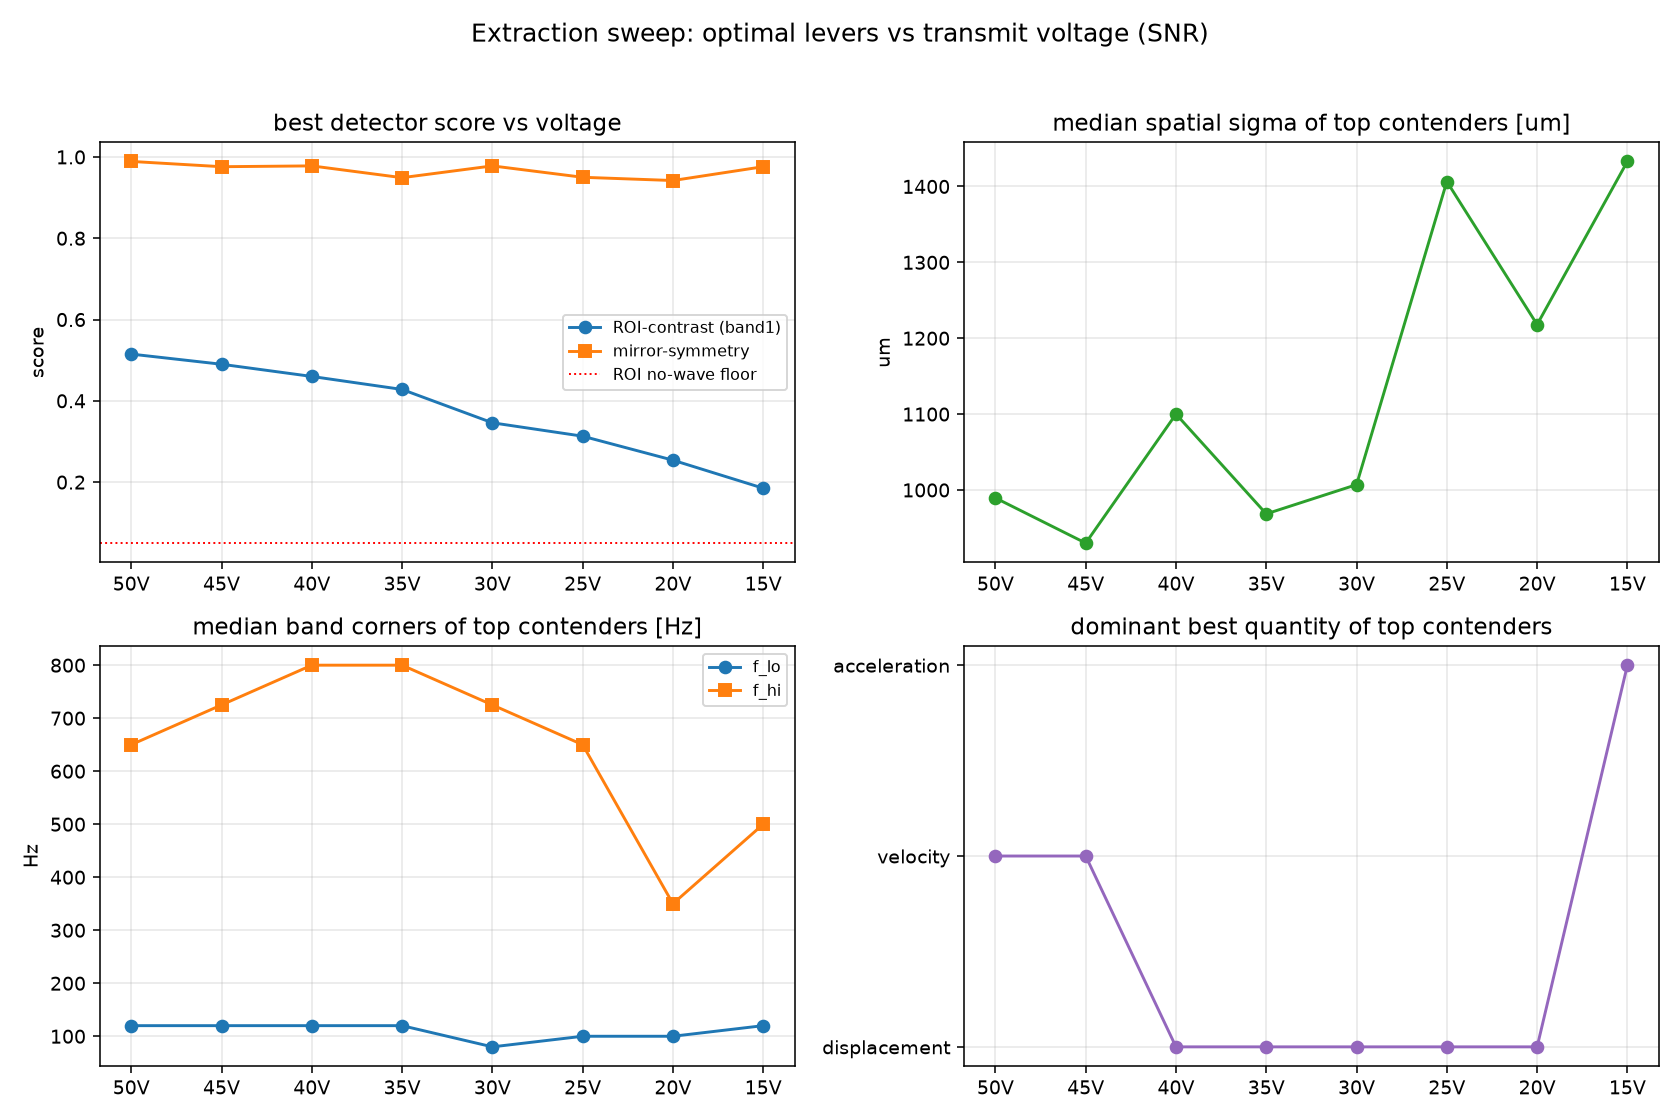
\includegraphics[width=\textwidth]{sweep_snr_trends.png}
  \caption{Optimal levers vs voltage.}
\end{subfigure}
\caption{Low-SNR extraction sweep. \emph{(a)} The symmetric V is recovered and rides the locked template at
every voltage down to 15\,V. \emph{(b)} As SNR drops the winners move to heavier Gaussian smoothing, a
narrower low-frequency band, and displacement --- there is no single fixed recipe.}
\label{fig:lowsnr}
\end{figure}

% ======================================================================
\section{Recommended acquisition changes for new in-vivo data}\label{sec:acq}
% ======================================================================
Motivated by the in-vivo failure (\S\ref{sec:invivo}) and the Caenen comparison, we ran a phantom
\textbf{acquisition-parameter sweep} (11 configurations $\times$ \{20, 30\}\,V, one-at-a-time over push
pulse length, push aperture, and tracking PRF) to find which \emph{acquisition} levers actually change the
space-time, and at what MI cost. Figure~\ref{fig:acq_montage} shows the resulting space-time for every
configuration --- the direct visual effect of increasing/decreasing pulse length, element count, PRF, and
their combination --- and Figure~\ref{fig:acq} quantifies it.

\begin{itemize}
  \item \good{Push aperture (F-number) is the dominant lever, monotonically.} 21$\rightarrow$79 push
  elements raises ROI-contrast $0.19\rightarrow0.44$ at 30\,V (symmetry $0.37\rightarrow0.91$): a
  clutter-filled panel becomes a crisp symmetric V.
  \item \textbf{Longer push pulse helps modestly and is ``free'' on MI} (peak pressure unchanged; only
  thermal/$I_\mathrm{spta}$ rises). A short pulse clearly hurts.
  \item \textbf{Tracking PRF is nearly negligible on the static phantom} (tracking is not the bottleneck on
  a static target) --- but it is expected to matter in vivo, where the wall moves, so it should be kept as a
  lever (a shallow wall-only high-PRF tracking window to avoid range-wrap).
  \item \textbf{Combinations are super-additive at low voltage} (max aperture $+$ long pulse roughly doubles
  the 20\,V base), which is exactly the low-SNR regime that matters in vivo.
  \item MI (coherent-sum estimate) is $\sim$linear in element count: $+48\%$ at 61 elements, $+90\%$ at 79.
\end{itemize}

\paragraph{Recommendation.} \good{Use $\sim$61 push elements and a $\sim$800\,\si{\micro s} pulse.} Sixty-one
elements captures nearly all of the aperture benefit (ROI 0.42 vs 79-element's 0.44 at 30\,V) for
\emph{half} the MI penalty ($+48\%$ vs $+90\%$); 79 elements buys only $+0.02$ ROI for nearly double the MI.
The longer pulse adds clarity at no MI cost, and the two should be super-additive at the low SNR that matters
in vivo. PRF can be left at base or raised modestly with a shallow tracking window. \caveat{Caveat:} these are
single-phantom rankings with a first-order (linear-acoustics) MI estimate; the aperture$\gg$pulse$\gg$PRF
\emph{ordering} is the transferable result, and one confirmatory 61-element$+$long-pulse acquisition is worth
doing (that exact combination was not tested; the tested combo used 79 elements).

\begin{figure}[p]
\centering
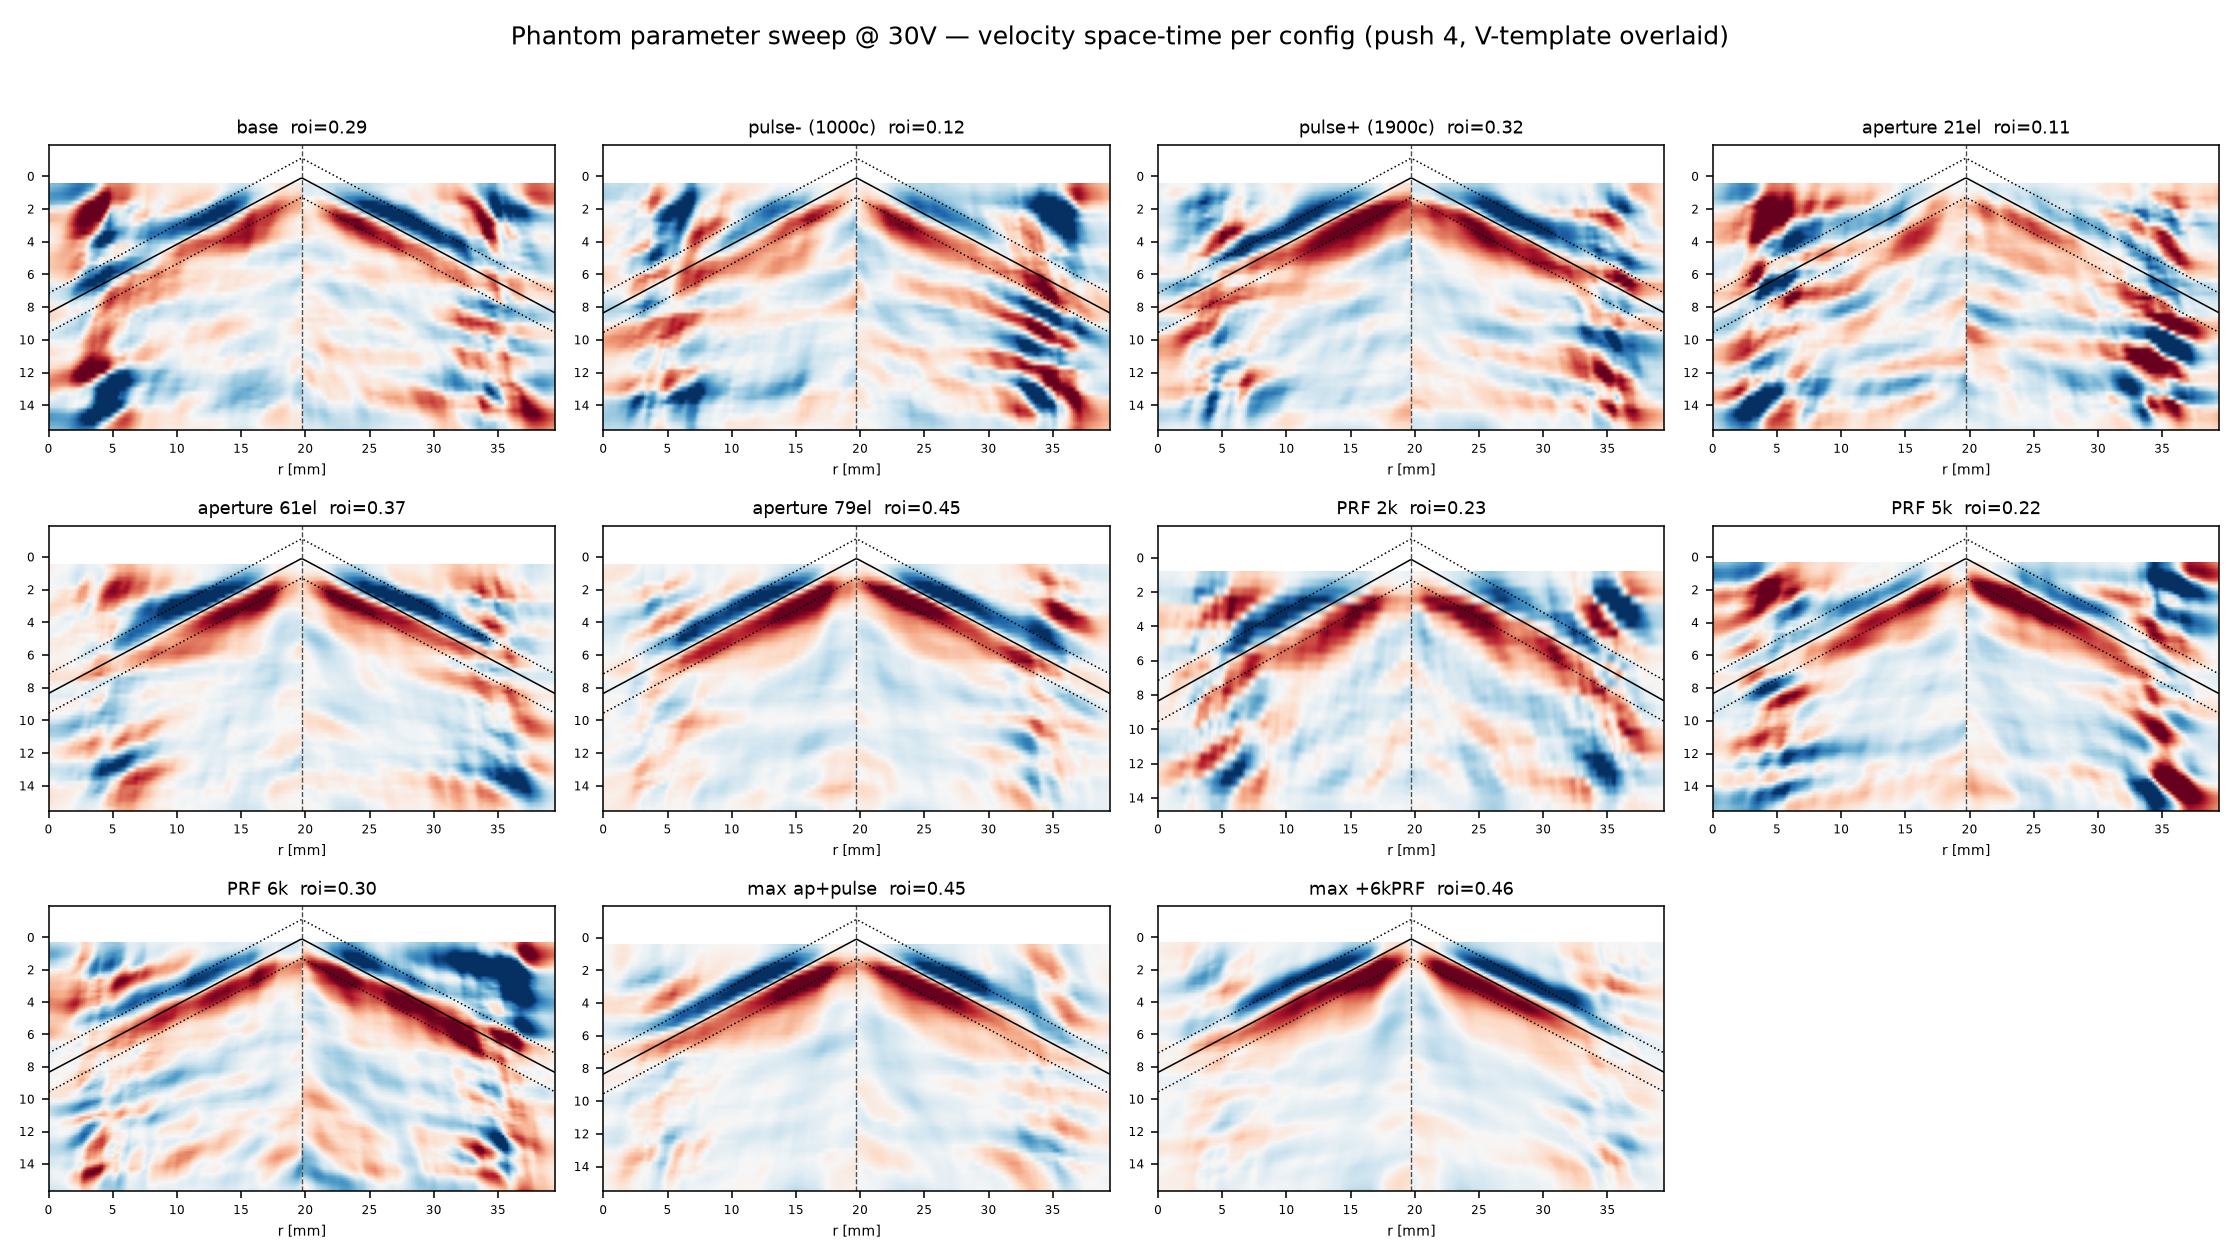
\includegraphics[width=\textwidth]{sweep_params_montage.png}
\caption{\textbf{The effect of each acquisition lever on the phantom shear-wave space-time} (velocity, at
30\,V, with the locked V-template overlaid). One panel per configuration, swept one-at-a-time from the
\emph{base} (1500 cycles / 41 elements / 3.7\,kHz):
\emph{Push pulse length} --- \texttt{pulse-} (1000\,cyc) $\rightarrow$ base $\rightarrow$ \texttt{pulse+}
(1900\,cyc): a short pulse is clearly worse, a longer pulse modestly better.
\emph{Number of push elements (aperture / F-number)} --- \texttt{21} $\rightarrow$ \texttt{41} (base)
$\rightarrow$ \texttt{61} $\rightarrow$ \texttt{79}: the dominant, monotonic lever, turning a
clutter-filled panel (\texttt{21 el}, ROI 0.11) into a crisp symmetric V (\texttt{79 el}, ROI 0.45).
\emph{Tracking PRF} --- \texttt{2\,kHz} $\rightarrow$ base $\rightarrow$ \texttt{5\,kHz} $\rightarrow$
\texttt{6\,kHz}: nearly negligible on a static phantom.
\emph{Combinations} --- \texttt{max ap+pulse} (79\,el $+$ 1900\,cyc) and \texttt{max +6kPRF}: the cleanest
Vs (ROI 0.45--0.46), super-additive at low voltage. ROI-contrast annotated per panel.}
\label{fig:acq_montage}
\end{figure}

\begin{figure}[t]
\centering
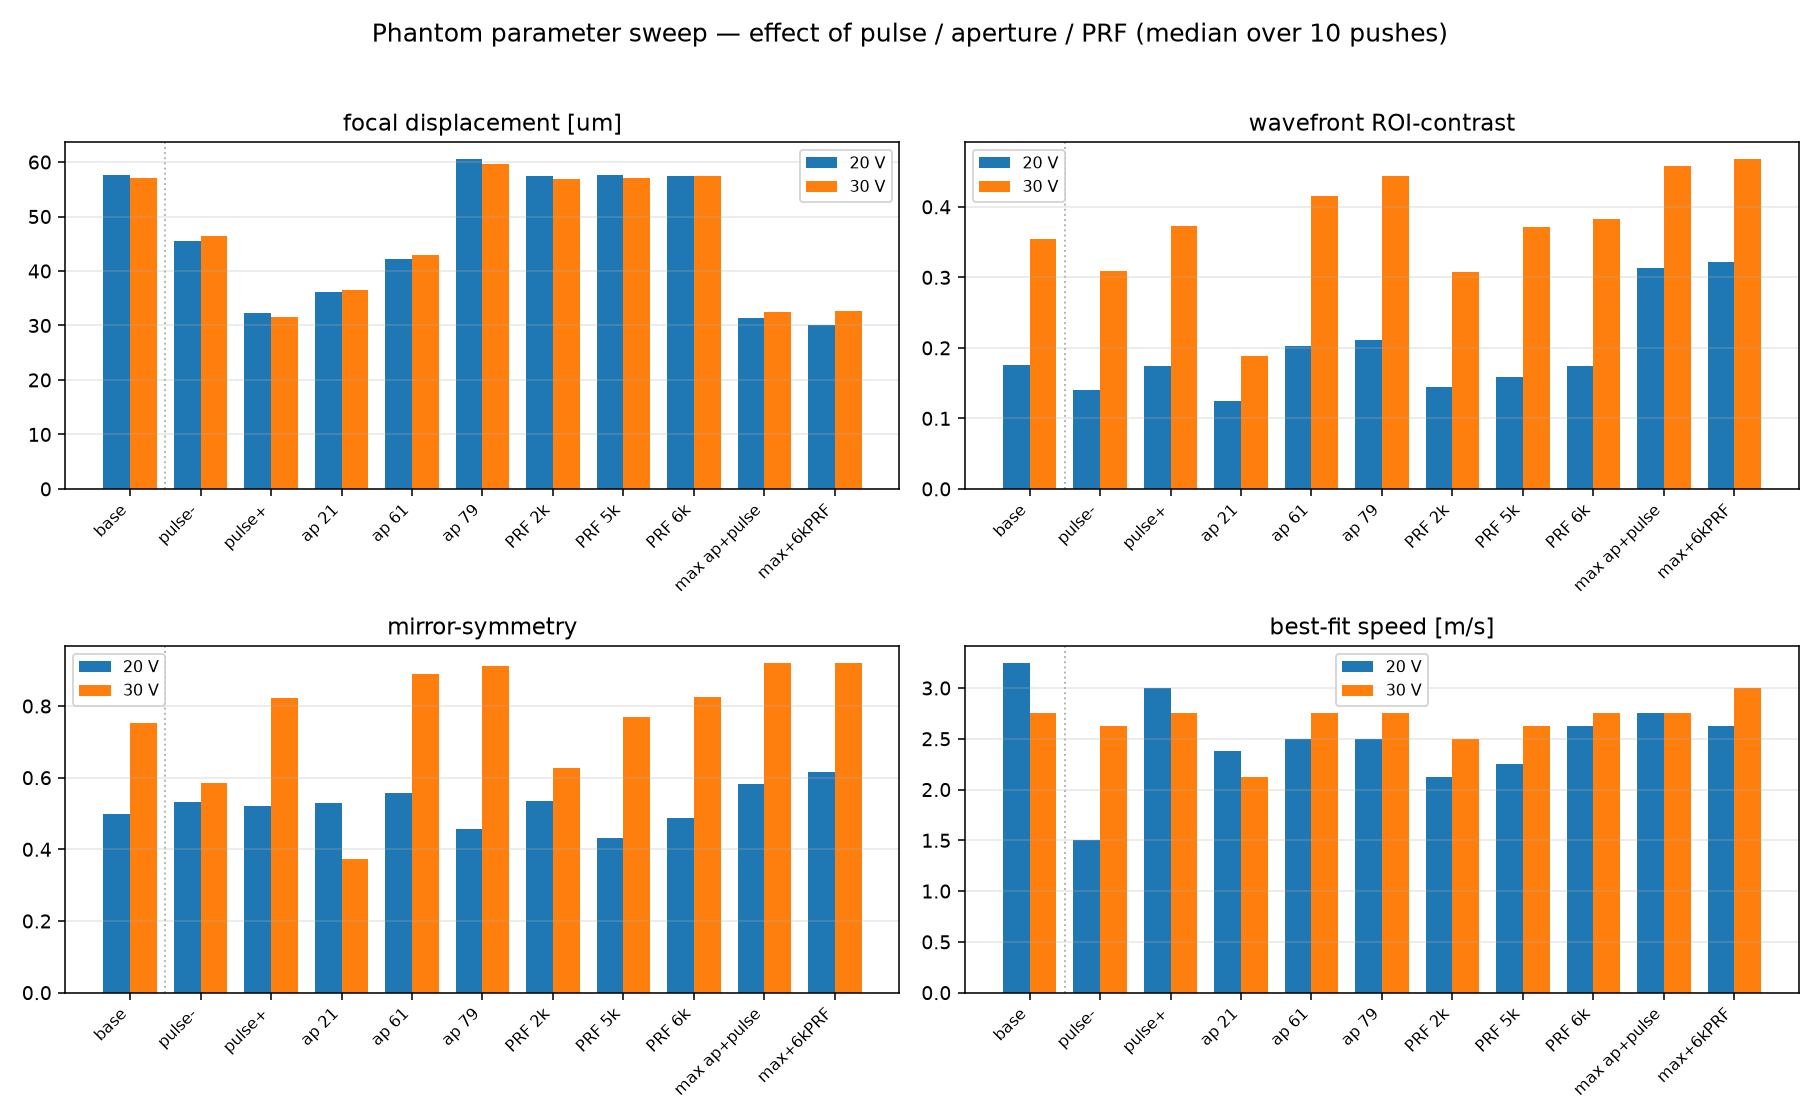
\includegraphics[width=0.95\textwidth]{sweep_params.png}
\caption{Metric bar charts quantifying Fig.~\ref{fig:acq_montage} (median over 10 pushes, 20\,V and 30\,V).
Aperture (F-number) is the dominant lever (ROI-contrast and symmetry rise monotonically with element count);
pulse length is a modest second; PRF is negligible on the static phantom; the measured speed
($\sim$2.5--3\,m/s) stays constant across all configs --- the levers change wavefront \emph{clarity}, not the
stiffness reading.}
\label{fig:acq}
\end{figure}

% ======================================================================
\section{Extracting shear waves from the Caenen pig data}\label{sec:caenen}
% ======================================================================
The Caenen pig dataset is the crucial external validation that our pipeline works on a \emph{real cardiac
ARF wave}. Running the full 52-push sweep (\texttt{sweep\_caenen.py}, $\sim$40\,min/push with resume
support), \good{a clean symmetric V is recovered at \emph{every} push} (52/52 with ROI-contrast $>0.25$;
ROI and symmetry cluster high together, Fig.~\ref{fig:caenen}) --- the clean opposite of the in-vivo
bulk-motion pile-up (\S\ref{sec:invivo}).

\good{The winning method combination follows the same family as the phantom}, which is reassuring evidence
that the pipeline is coherent across data sources (Fig.~\ref{fig:caenen_methods}): a band-pass with a
\emph{high low-corner ($\sim$120\,Hz) is decisively best} (ROI 0.46 vs 0.28 at 10--40\,Hz --- the single
dominant lever, mirroring the passive-SWE finding that bulk wall motion must be removed by a
$\geq\!\sim$10--20\,Hz corner), a narrow 120--350\,Hz band, median$\approx$Gaussian smoothing (NLM worst),
and --- because this wave is \emph{clean} (high SNR) --- \emph{acceleration} is the best quantity
(0.37 vs velocity 0.30 vs displacement 0.18), exactly the SNR-dependent quantity shift the phantom study
predicted. Light SVD-2 IQ clutter helps mildly.

\begin{figure}[t]
\centering
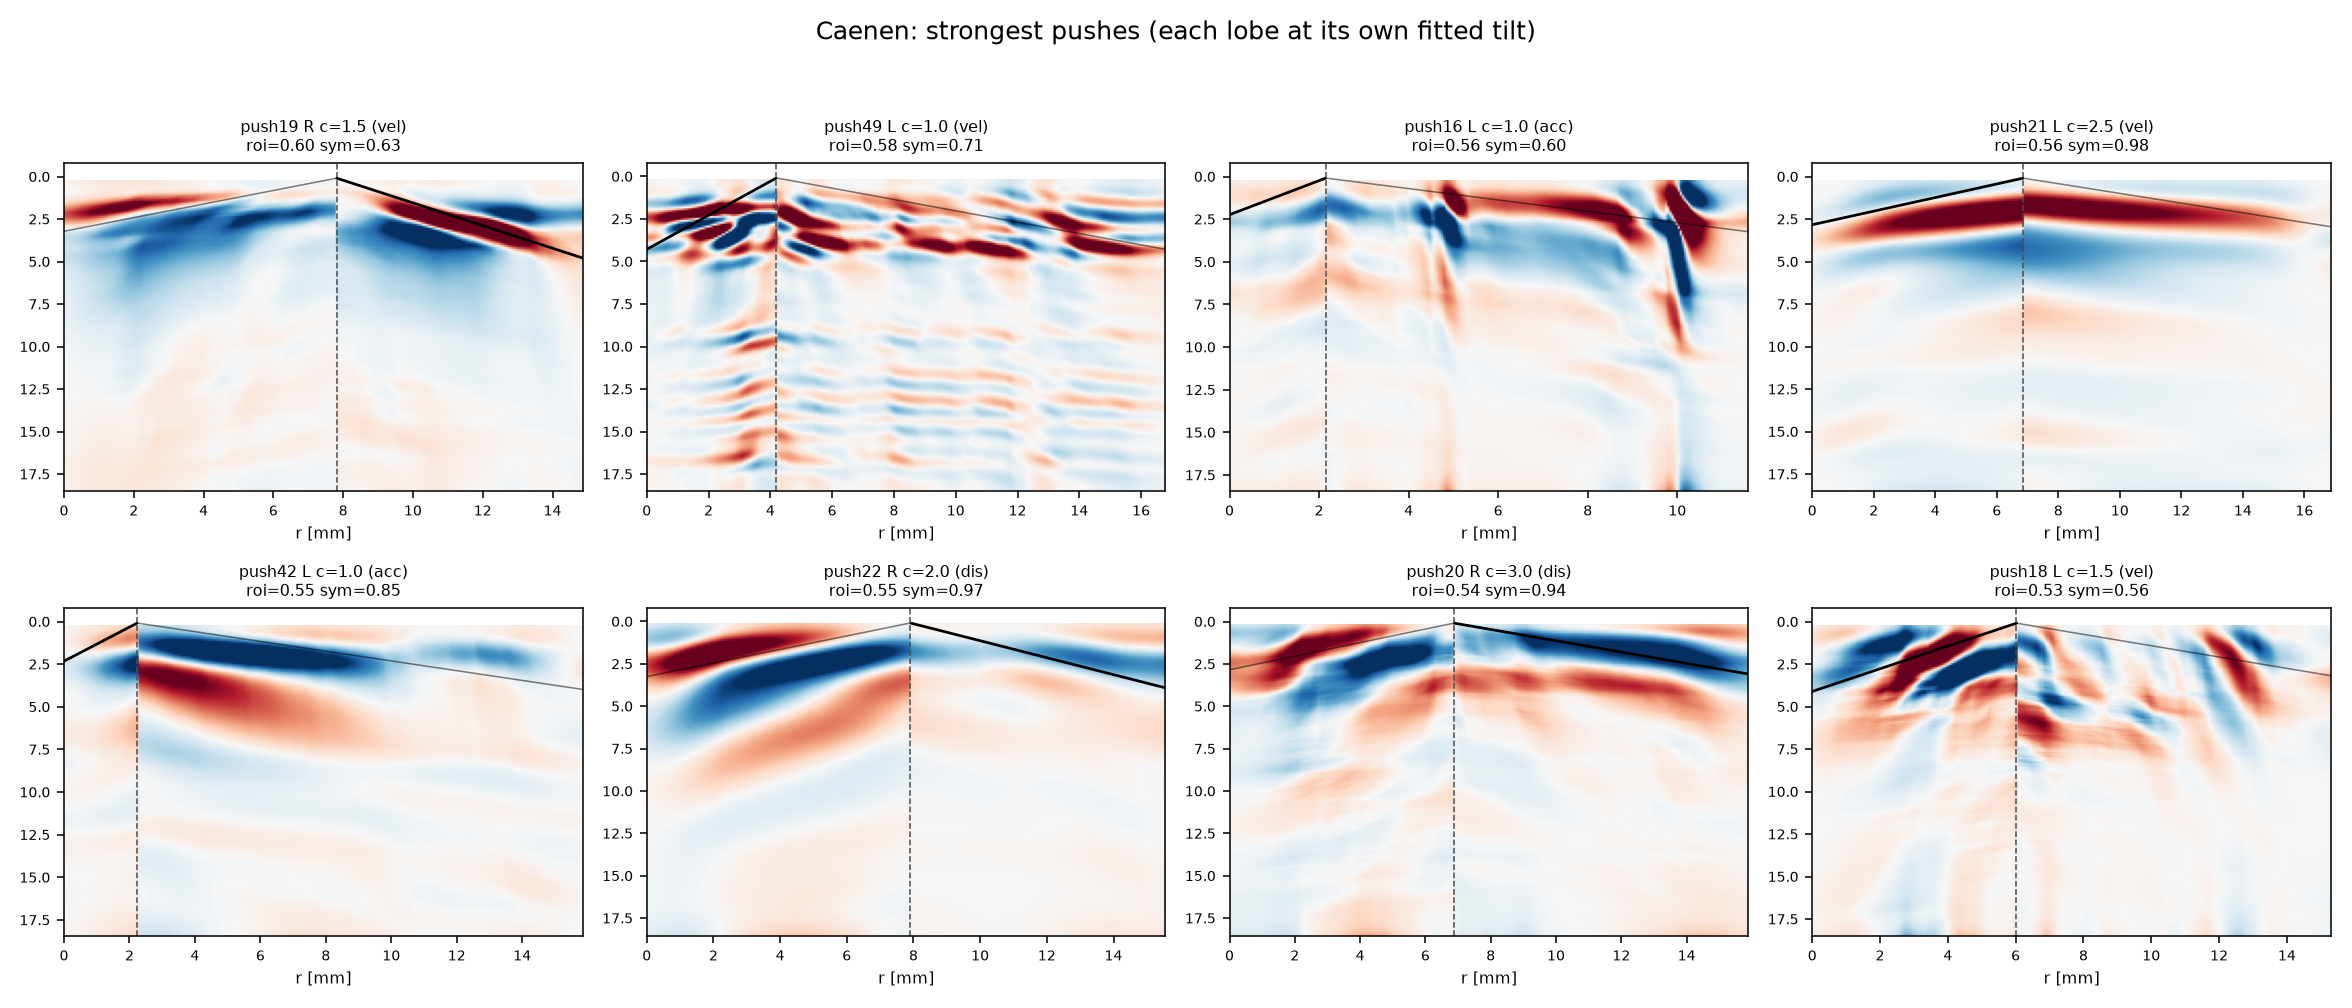
\includegraphics[width=\textwidth]{caenen_montage.png}
\caption{Caenen pig ARF-SWE: the eight strongest pushes, each lobe drawn at its own best-fit tilt (the
oblique septum is not mirror-symmetric). A clean propagating wavefront is recovered in displacement,
velocity and acceleration; ROI-contrast and symmetry are annotated per panel. This is a \emph{real cardiac
ARF wave}, recovered by the same pipeline used on the phantom.}
\label{fig:caenen}
\end{figure}

\begin{figure}[t]
\centering
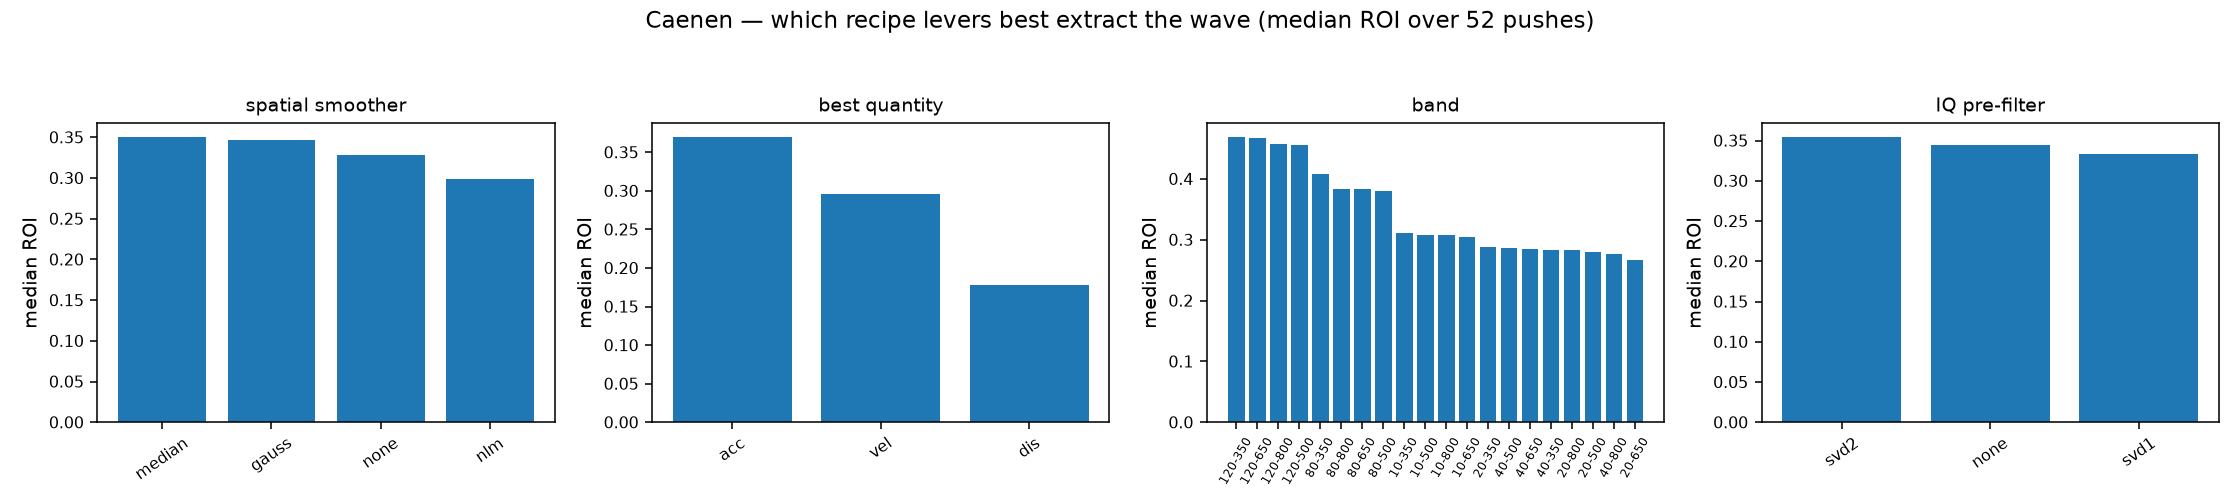
\includegraphics[width=\textwidth]{caenen_methods.png}
\caption{Caenen: which recipe levers best extract the wave (median ROI over 52 pushes). The winners match
the phantom/passive family: a high band low-corner ($\sim$120\,Hz) is decisive, a narrow 120--350\,Hz band
is best, median$\approx$Gaussian smoothing beats NLM, and --- for this clean, high-SNR wave ---
\emph{acceleration} is the best quantity.}
\label{fig:caenen_methods}
\end{figure}

\caveat{One important caveat on speed.} The 52 pushes span $\sim$1.8 cardiac cycles, so the per-push
best-fit speeds (spread $\sim$1.5--5\,m/s, mostly clustered 2--3\,m/s; Fig.~\ref{fig:caenen_speed}) reflect
genuine \emph{systolic/diastolic stiffness modulation} and must \emph{not} be pooled into one mean SWS.
A systolic-vs-diastolic fit needs the ECG timing (as in the Caenen paper's piecewise model); the
\emph{extraction quality} (ROI/symmetry) is poolable and is what the method study above uses.

\begin{figure}[t]
\centering
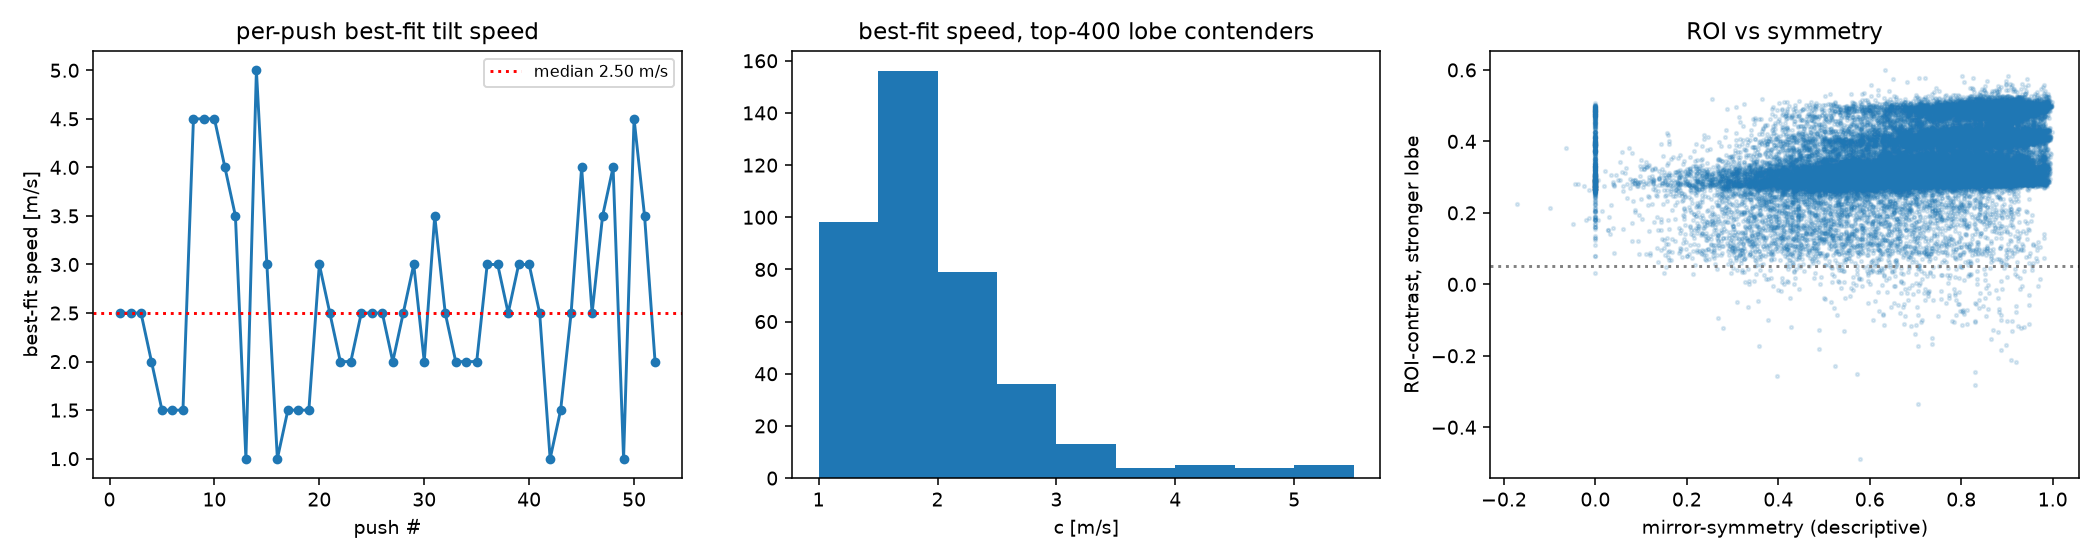
\includegraphics[width=\textwidth]{caenen_speed_overview.png}
\caption{Caenen speed overview. \emph{Left:} per-push best-fit tilt speed varies over the cardiac cycle
(this modulation is physiological and should not be averaged away). \emph{Middle:} best-fit speed
distribution clusters at 2--3\,m/s. \emph{Right:} ROI-contrast rises with mirror-symmetry --- a real,
consistent wave.}
\label{fig:caenen_speed}
\end{figure}

\paragraph{The positive control the in-vivo data lacks.} To make the contrast with our in-vivo data
explicit, Figure~\ref{fig:caenen_pushnopush} runs the \emph{same push/no-push montage} as the in-vivo
Figure~\ref{fig:allpush}, but on all 52 Caenen pushes: each push's tracking space-time above its own
pre-push no-push control, identical pipeline machinery. Processed with the Caenen-tuned recipe (velocity,
narrow 120--350\,Hz band --- the high-SNR reading of the same SNR-adaptive recipe, \S\ref{sec:scoring}),
\good{every one of the 52 push panels shows a strong, coherent wave} (\texttt{origin\_coherence}
$\approx$0.98 across the board), and the push exceeds its own no-push control in $\approx$85\% of pushes.
The no-push controls are \emph{not} always silent --- the pig heart also moves, and
\texttt{origin\_coherence} is permissive (exactly the caveat from \S\ref{sec:invivo}) --- but the decisive
difference is that here the push \emph{reliably} adds the propagating wavefront on top, whereas in vivo
(Fig.~\ref{fig:allpush}) it rarely rose above its control. (A few pushes read \texttt{oc}$=$0 where the
push sits at the very end of the M-line and the symmetric coherence metric degenerates --- a known
limitation of that metric, not a missing wave; the wavefront is still visible in those panels.) This is
the clean positive control: the same pipeline, applied to a genuinely stronger, shallower, ECG-gated push,
recovers the wave \emph{every time} --- which is precisely what the in-vivo acquisition changes
(\S\ref{sec:next}) aim to reproduce.

\begin{figure}[p]
\centering
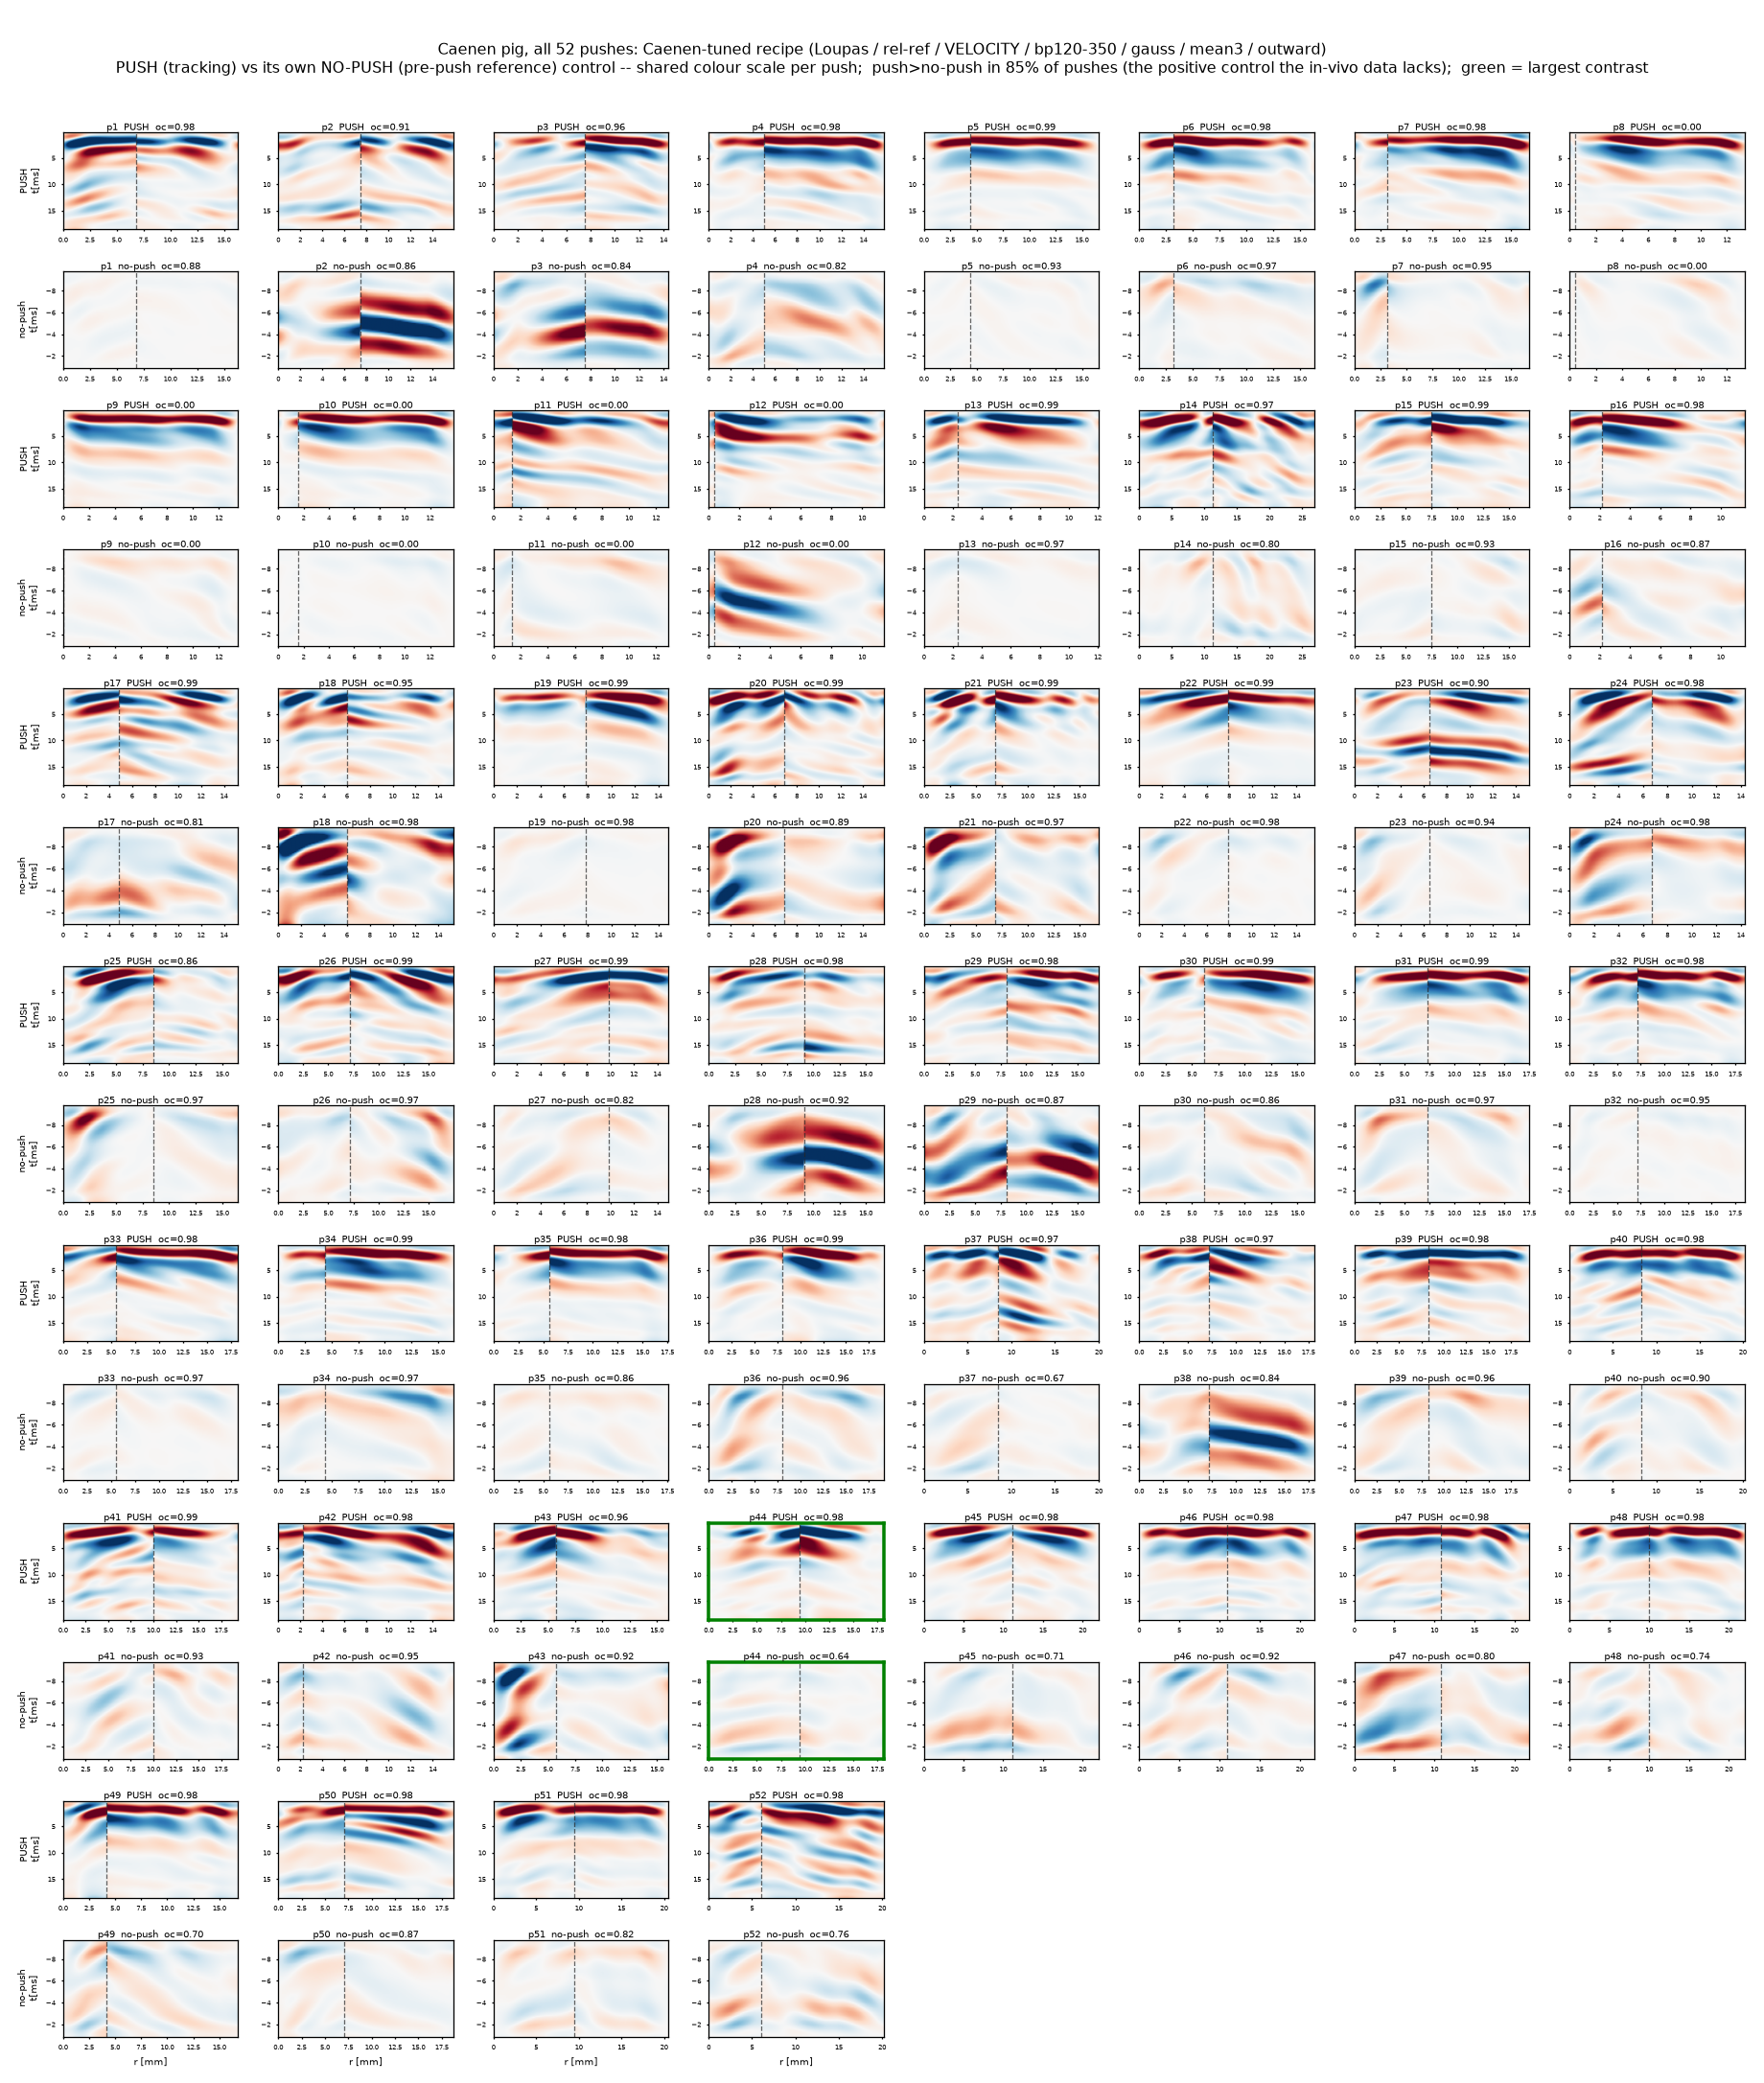
\includegraphics[width=\textwidth]{caenen_push_nopush_montage.png}
\caption{The push/no-push montage of Fig.~\ref{fig:allpush}, applied to \textbf{all 52 Caenen pig pushes}
with the Caenen-tuned recipe (Loupas / relative-to-reference / \emph{velocity} / band-pass 120--350\,Hz /
Gaussian smooth / moving-mean / outward / 7 offsets). Each push's post-push \emph{tracking} space-time
(``PUSH'' rows) sits above its own pre-push \emph{no-push} control, shared colour scale per push, dashed
line $=$ push origin $r_0$, \texttt{origin\_coherence} annotated per panel. Every push panel shows a
strong coherent wave (\texttt{oc}$\approx$0.98) and the push exceeds its no-push control in $\approx$85\%
of pushes --- the positive control the in-vivo data (Fig.~\ref{fig:allpush}) lacks. \textbf{p44} (green)
has the largest push-vs-no-push contrast ($+0.34$).}
\label{fig:caenen_pushnopush}
\end{figure}

% ======================================================================
\section{Why we (so far) fail to extract shear waves from the in-vivo human data}\label{sec:invivo}
% ======================================================================
This is the project's clear negative result, and it is well-supported. \caveat{Our current in-vivo human
data does not contain a recoverable ARF shear wave: the active space-time plots are dominated by cardiac
wall motion, not the push.} The evidence is threefold and mutually consistent:

\begin{enumerate}
  \item \textbf{Voltage has no effect in vivo} (unlike the phantom). Raising the push 30\,$\rightarrow$40\,V
  did not make the wave clearer or stronger --- \texttt{origin\_coherence} and wave amplitude were
  statistically indistinguishable --- which is impossible for a genuine ARF push that scales with voltage on
  the phantom.
  \item \textbf{Amplitude and reality check.} The raw focal displacement in vivo is $\sim$42\,\si{\micro m},
  voltage-independent, and $\sim$$10\times$ the phantom push --- consistent with bulk cardiac wall motion,
  not a few-micron ARF impulse.
  \item \textbf{The no-push control is decisive} (Fig.~\ref{fig:nopush}). Running the identical recipe on the
  \emph{pre-push reference} window --- where no push fired --- still produces a coherent space-time in vivo
  (\texttt{origin\_coherence} 0.80), with \emph{horizontal in-phase bands} (the whole wall moving together)
  that are \emph{larger} than in the push window. On the phantom the reference is correctly quiet. In other
  words, the ``clean wave'' the pipeline draws in vivo can be manufactured from motion alone.
\end{enumerate}

Aggregated over all 24 pushes (Fig.~\ref{fig:pushnopush}), the push adds essentially no band-passed
amplitude over the pre-push reference (median ratio $\approx$1): most points sit on or below the
``push $=$ no-push'' diagonal.

\begin{figure}[t]
\centering
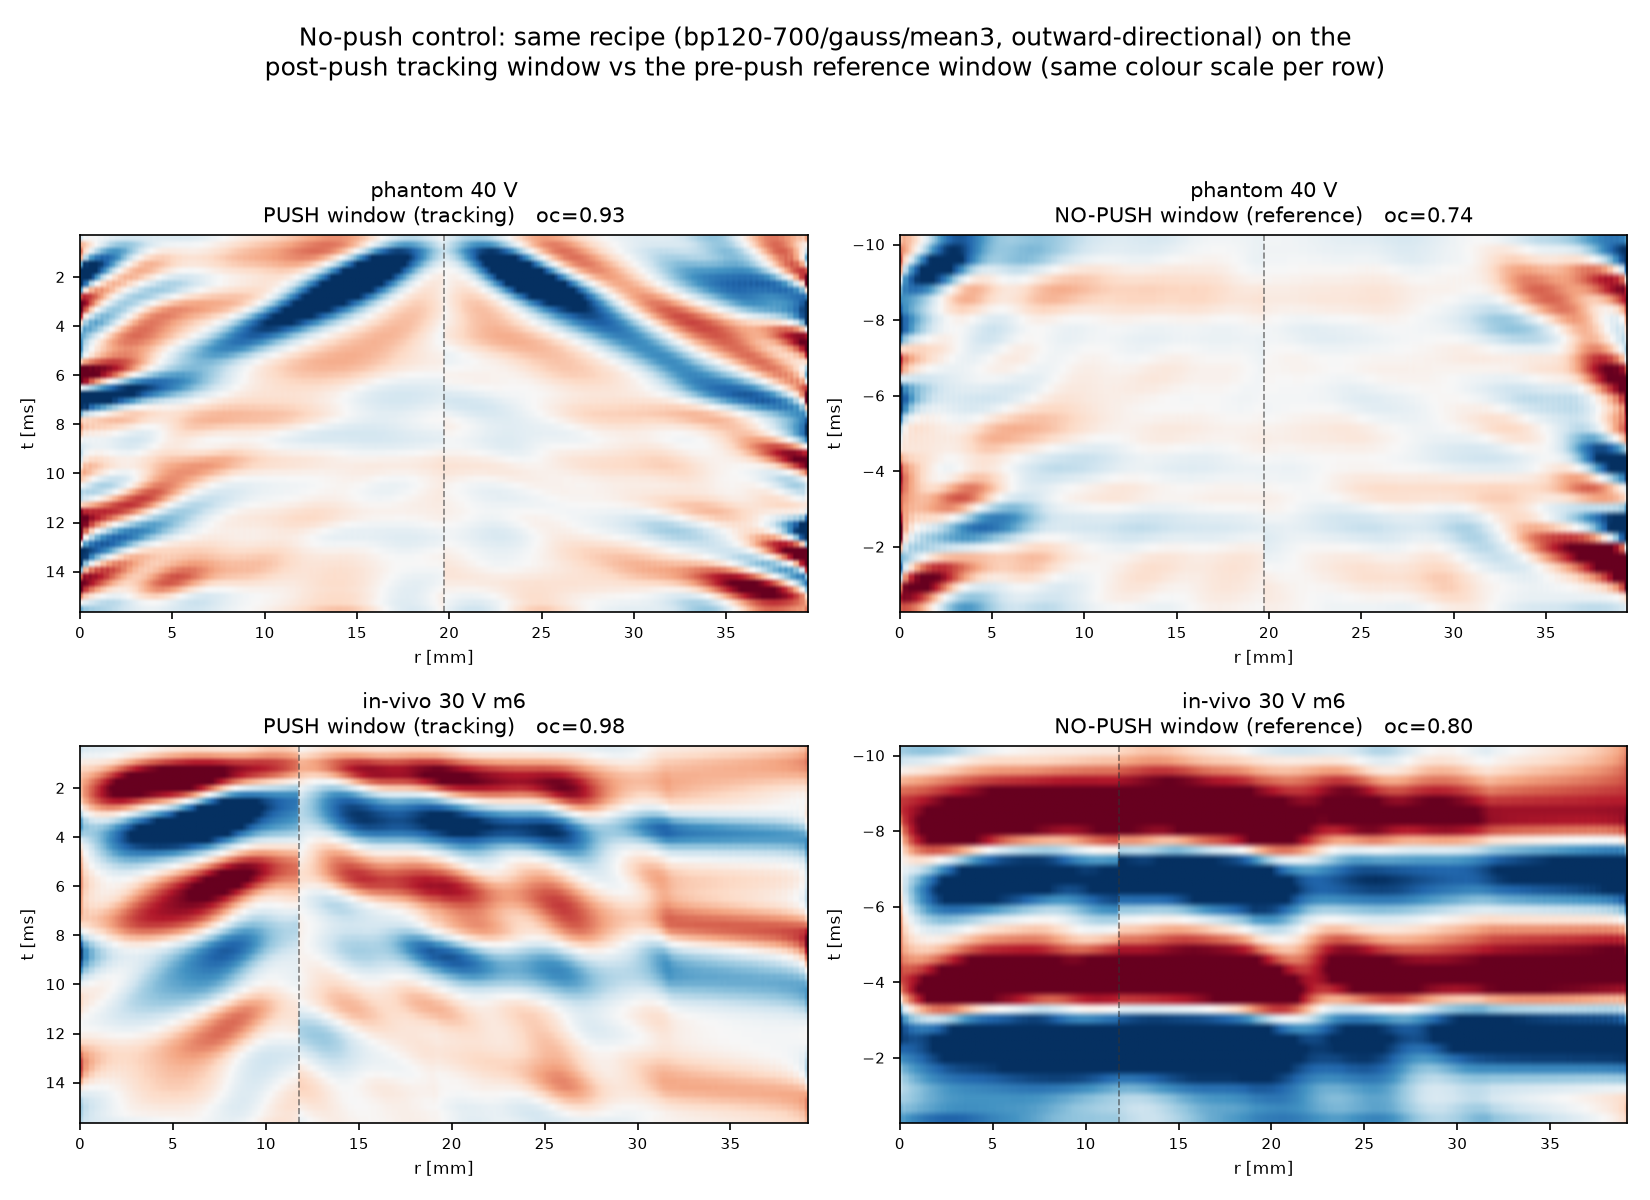
\includegraphics[width=0.92\textwidth]{nopush_control.png}
\caption{The decisive no-push control. The identical recipe is run on the post-push \emph{tracking} window
(left) and the pre-push \emph{reference} window (right). \emph{Phantom (top):} the reference is quiet
(oc\,0.74 with no structure) --- the push adds the wave. \emph{In vivo (bottom):} the reference shows strong
\emph{horizontal} in-phase bands (oc\,0.80) that are \emph{larger} than the push window --- the ``wave'' is
bulk cardiac motion, not the ARF push.}
\label{fig:nopush}
\end{figure}

\begin{figure}[t]
\centering
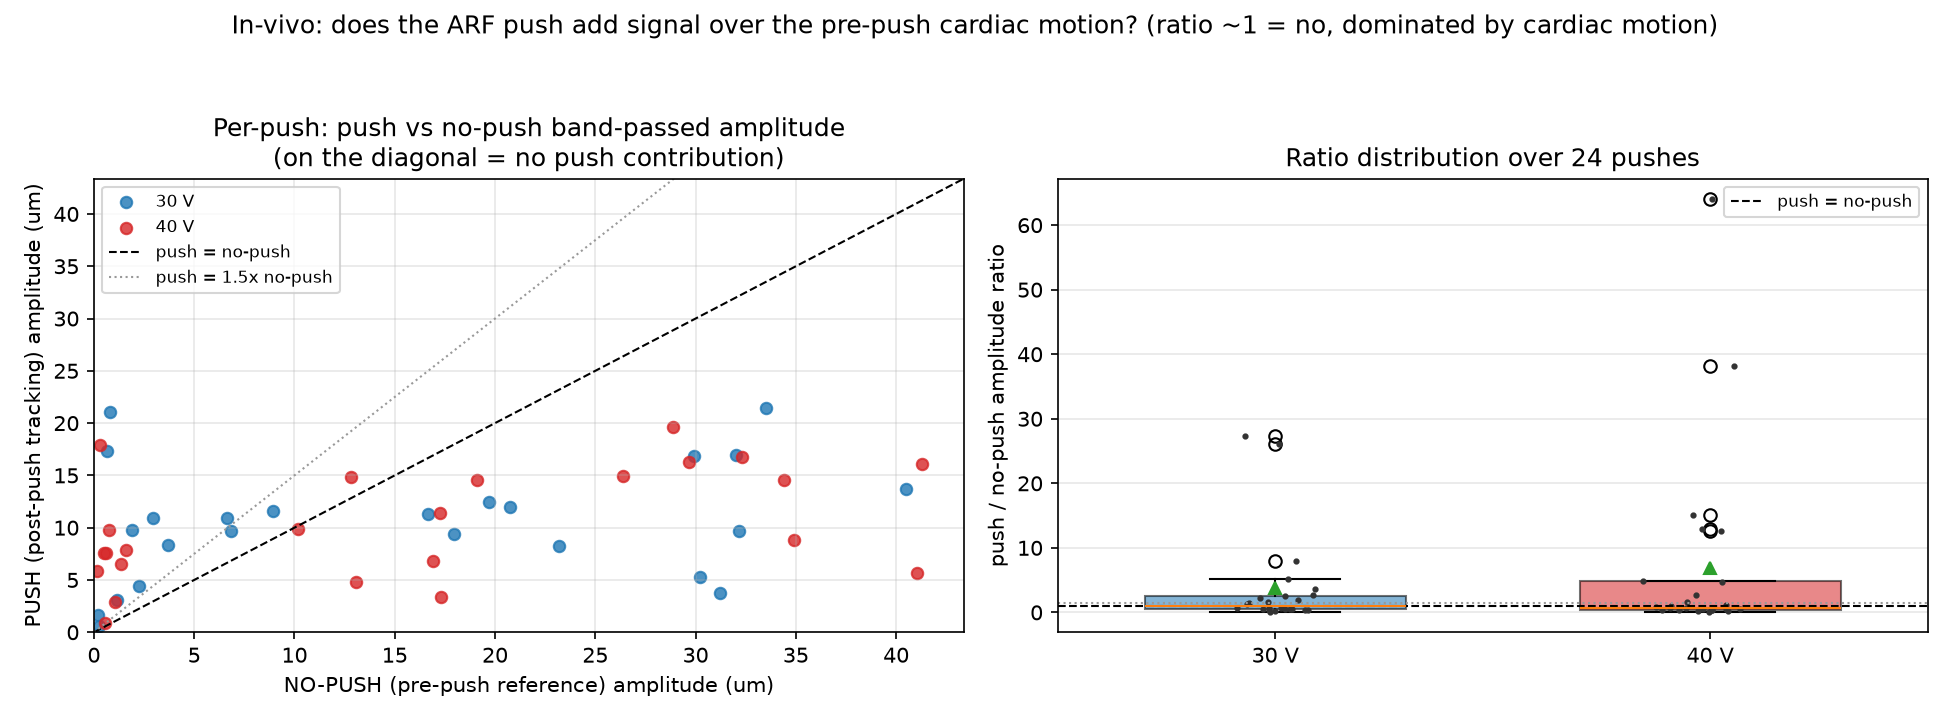
\includegraphics[width=0.92\textwidth]{push_vs_nopush_all.png}
\caption{All 24 in-vivo pushes. Post-push band-passed amplitude vs pre-push reference amplitude: points on
the diagonal mean the push added nothing over the pre-existing cardiac motion. At both 30\,V and 40\,V the
median ratio is $\approx$1 --- confirming the tracking ``signal'' is cardiac motion.}
\label{fig:pushnopush}
\end{figure}

\paragraph{Every push, side by side --- is there a wave in \emph{any} of them?} To make the
per-push picture concrete, Figure~\ref{fig:allpush} runs the settled optimal band-pass recipe on
\emph{all 24} pushes and shows each one's post-push (tracking) space-time directly above its own no-push
(pre-push reference) control, on a shared colour scale. The result is nuanced rather than uniformly
negative:
\begin{itemize}
  \item \textbf{The majority are cardiac-motion-dominated:} the push and no-push panels are \emph{both}
  strong, and the no-push shows the tell-tale near-horizontal in-phase bands of whole-wall motion
  (e.g.\ m0, m1, m3, m10, m11, m17, m20, m21) --- no push-specific wave.
  \item \good{A handful of quiet-phase (diastasis) pushes are the real candidates.} In m5, m6, m19 and m23
  the no-push control is genuinely \emph{quiet} (little pre-push motion), yet the push window carries more
  coherent structure --- a positive push-vs-no-push \texttt{origin\_coherence} contrast up to $+0.26$
  (m19: 0.99 vs 0.73; m23: 0.88 vs 0.61). These are exactly the pushes independently flagged as the
  quietest by pre-push wall-motion RMS, i.e.\ those landing near diastasis --- which is where a weak ARF
  transient has the best chance of peeking above the cardiac floor.
  \item \caveat{But even the best candidate is not a clean wave.} None of these panels shows the
  unambiguous, symmetric outward V that the phantom (Fig.~\ref{fig:voltage}) and the Caenen pig
  (Fig.~\ref{fig:caenen}) produce; the structure is weak, partly one-sided, and not clearly propagating.
  The honest reading is \emph{suggestive, not conclusive}: consistent with an underpowered push
  occasionally emerging at the quietest cardiac phase, but not a confident shear-wave detection.
\end{itemize}
This both answers the question directly --- \emph{if} any push contains a recoverable wave it is one of
the quiet-diastasis pushes --- and reinforces the diagnosis: it takes the quietest possible cardiac phase
for our current push to even approach visibility, which is what a stronger, ECG-gated push
(\S\ref{sec:next}) is designed to fix.

\begin{figure}[p]
\centering
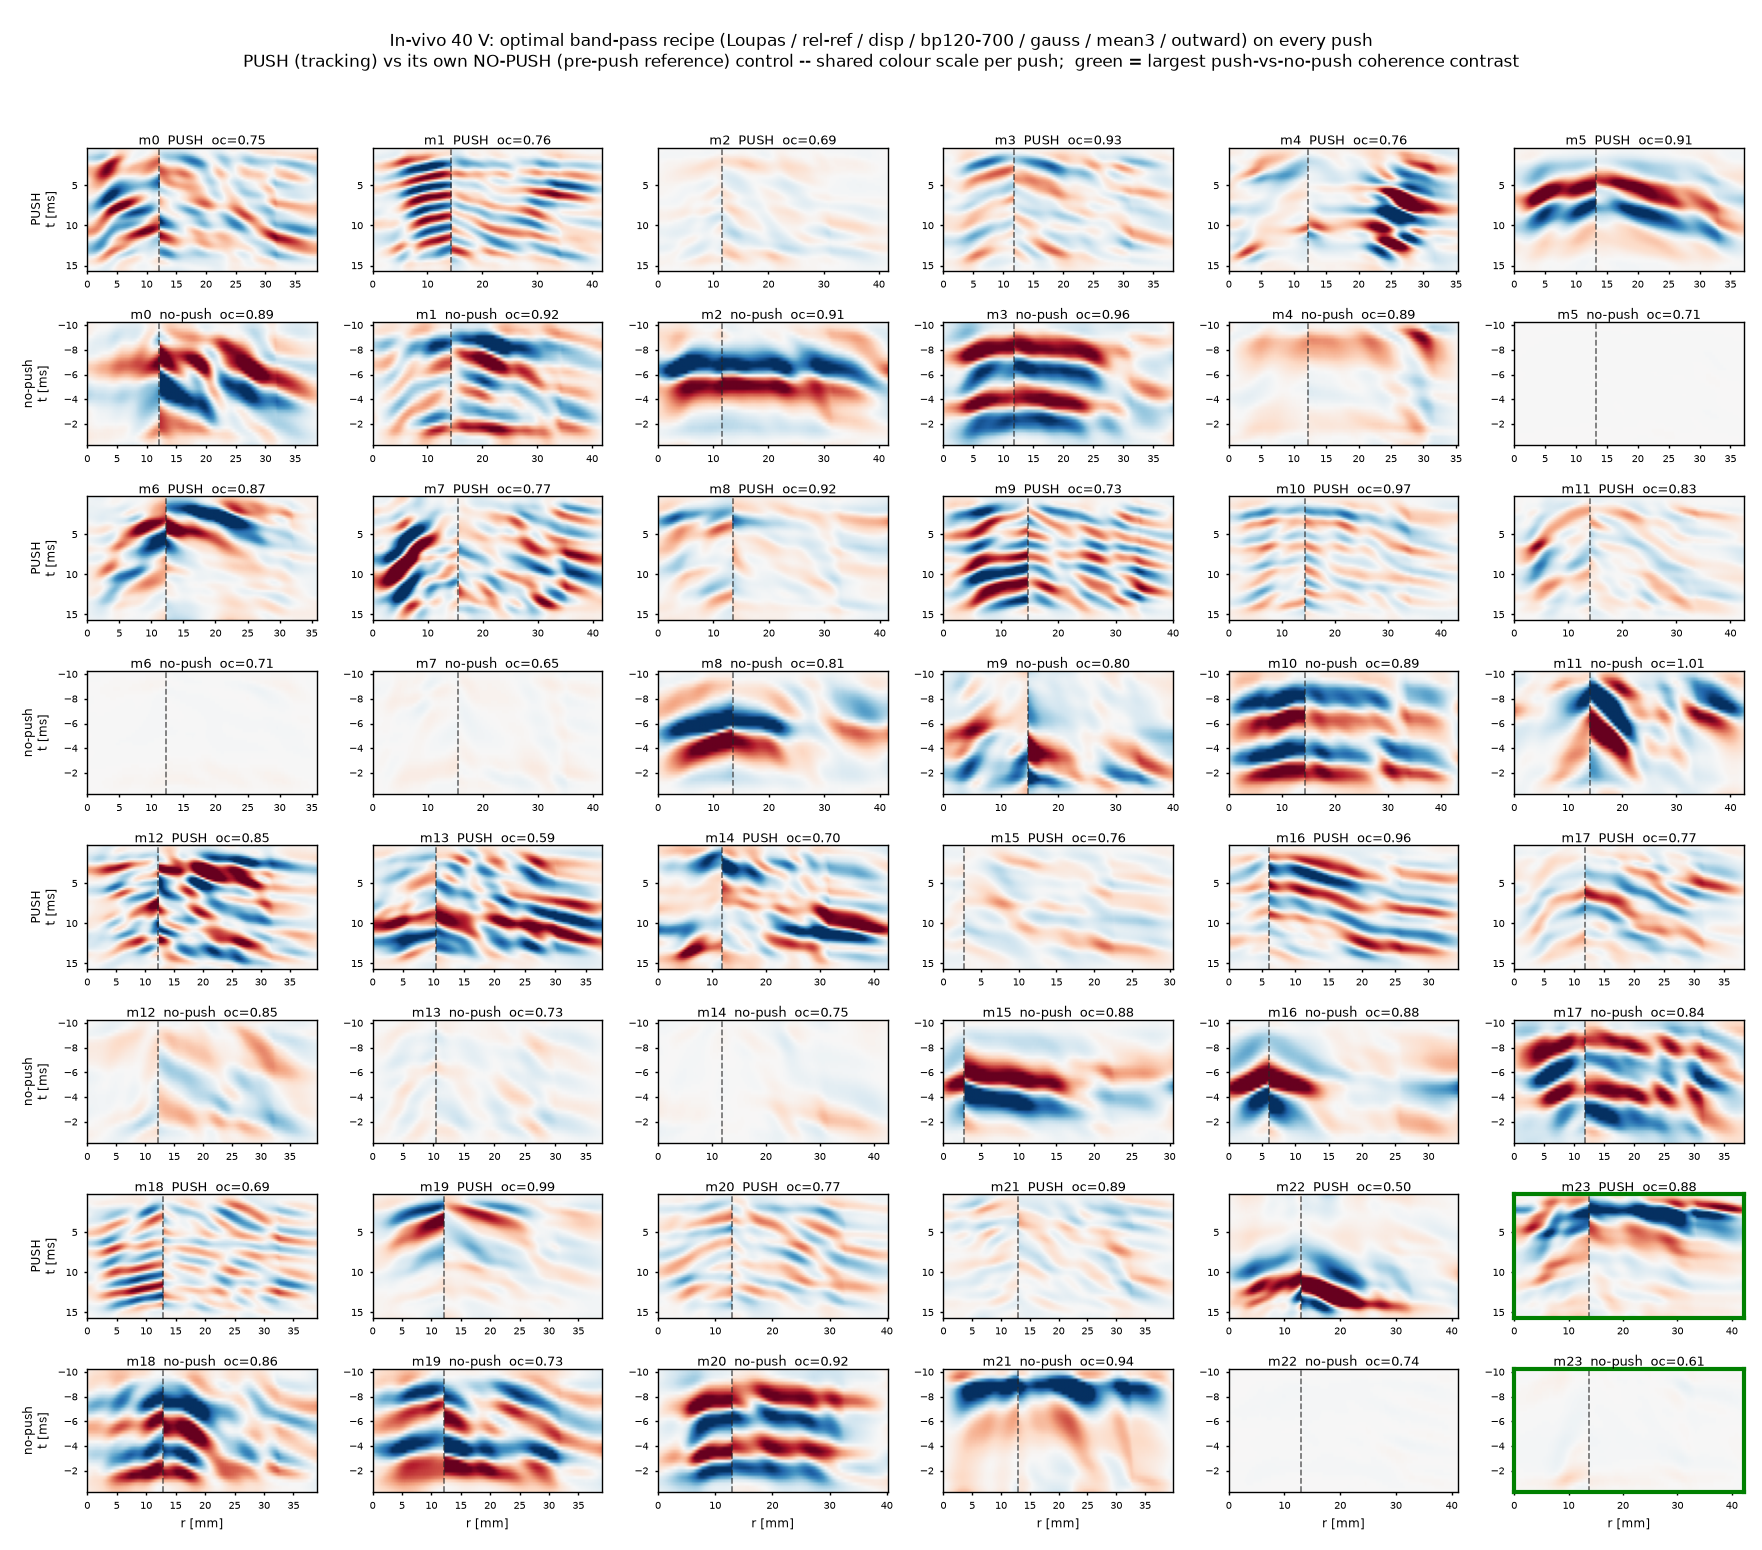
\includegraphics[width=\textwidth]{invivo40_push_nopush_montage.png}
\caption{The optimal band-pass recipe (Loupas / relative-to-reference / displacement / band-pass
120--700\,Hz / Gaussian smooth / moving-mean / outward-directional / 7 offsets) applied to \textbf{all 24
in-vivo 40\,V pushes}. Each push shows its post-push \emph{tracking} space-time (``PUSH'' rows) directly
above its own pre-push \emph{no-push} control, on a shared colour scale per push; the dashed line is the
push origin $r_0$ and \texttt{origin\_coherence} is annotated per panel. Most pushes are cardiac-motion
dominated (strong, horizontally-banded no-push controls). The four quiet-diastasis pushes (m5, m6, m19,
m23) have quiet no-push controls and the largest push-vs-no-push coherence contrast --- the only
candidates for a captured wave; \textbf{m23} (green) has the largest contrast ($+0.26$). Even these fall
short of the clean symmetric V seen on the phantom and Caenen data.}
\label{fig:allpush}
\end{figure}

\paragraph{The no-push control and its data-leakage trap.} A subtlety makes the no-push control both
trustworthy and non-trivial. For recipes whose steps are \emph{not fitted to} the reference (band-pass,
smoothing, SVD on the tracking movie), the control simply runs the identical recipe on the pre-push
reference window --- there is nothing to leak. But several of the strongest cardiac-motion removers
(reference polynomial extrapolation, reference-subspace projection, adaptive high-pass) \emph{train} their
model on the pre-push frames and subtract it. If such a filter were then evaluated on that same reference
window, it would be scored on its own training data --- trivially annihilating (or fabricating) structure,
telling us nothing. The harness therefore uses a \textbf{held-out / split reference}
(\texttt{motion\_removal.py}): the pre-push frames are split in half, the filter is trained on the first
half and evaluated on the disjoint second half (guaranteed push-free), exactly mirroring the real
experiment (train on the full reference, apply to the tracking window) but with a test window that cannot
contain a wave. This is fair because cardiac motion is quasi-periodic, so the first half predicts the
second --- the same assumption the reference filter relies on in the real case. It is precisely this
leakage-free control that exposed reference-subspace projection and SVD clutter \emph{fabricating} a false
V from pure motion.

\paragraph{Root cause: acquisition-limited.} The comparison with Caenen
(Table~\ref{tab:data}; \texttt{docs/caenen\_vs\_invivo\_acquisition.md}) pinpoints \emph{why}. Our push is
\emph{much weaker and worse-placed}: F/$\approx$4.3 at 44.6\,mm and 40\,V, versus Caenen's F/1 at 25\,mm and
50--60\,V. ARF scales with beam intensity, a tighter F-number concentrates energy, and a shallower focus
suffers less attenuation --- so Caenen displaces the wall by many microns while our loose, deep,
lower-voltage push produces a vibration that falls below the 20--40\,\si{\micro m} of cardiac motion. Our
small S5-1 footprint simply cannot form an F/1 push at 44.6\,mm. Compounding this, we track at half the
frame rate (3.7 vs 8.8\,kHz), at twice the depth, and \emph{free-running} (pushes land at arbitrary,
often fast-moving cardiac phases) rather than R-peak-triggered. Notably, our \emph{processing} is not the
weak point --- we already use Loupas, the paper's own recommended upgrade over Kasai, and the same pipeline
recovers the Caenen wave cleanly.

\paragraph{Processing cannot manufacture the wave --- and forcing it fabricates artifacts.} A dedicated
cardiac-motion-removal harness (\texttt{motion\_removal.py}), validated with a split-reference no-push
control, delivered a sobering but important negative (Fig.~\ref{fig:motionremoval}): \caveat{reference-subspace
projection and SVD clutter can \emph{fabricate} a false shear-wave ``V'' from pure cardiac motion} (high
no-push ROI on the quietest pushes) --- the no-push control catches exactly what a naive image metric would
miss. No method beat a plain band-pass, and every \emph{honest} motion-remover that quiets the reference also
suppresses the tracking signal --- because the tracking ``signal'' \emph{is} the cardiac motion. The one
best-behaved aggressive remover found (optical-flow compensation) quiets the reference without fabricating a
wave and is worth carrying forward, but on this acquisition-limited data nothing recovers a wave. This
confirms the diagnosis: the fix is acquisition, not processing.

\begin{figure}[t]
\centering
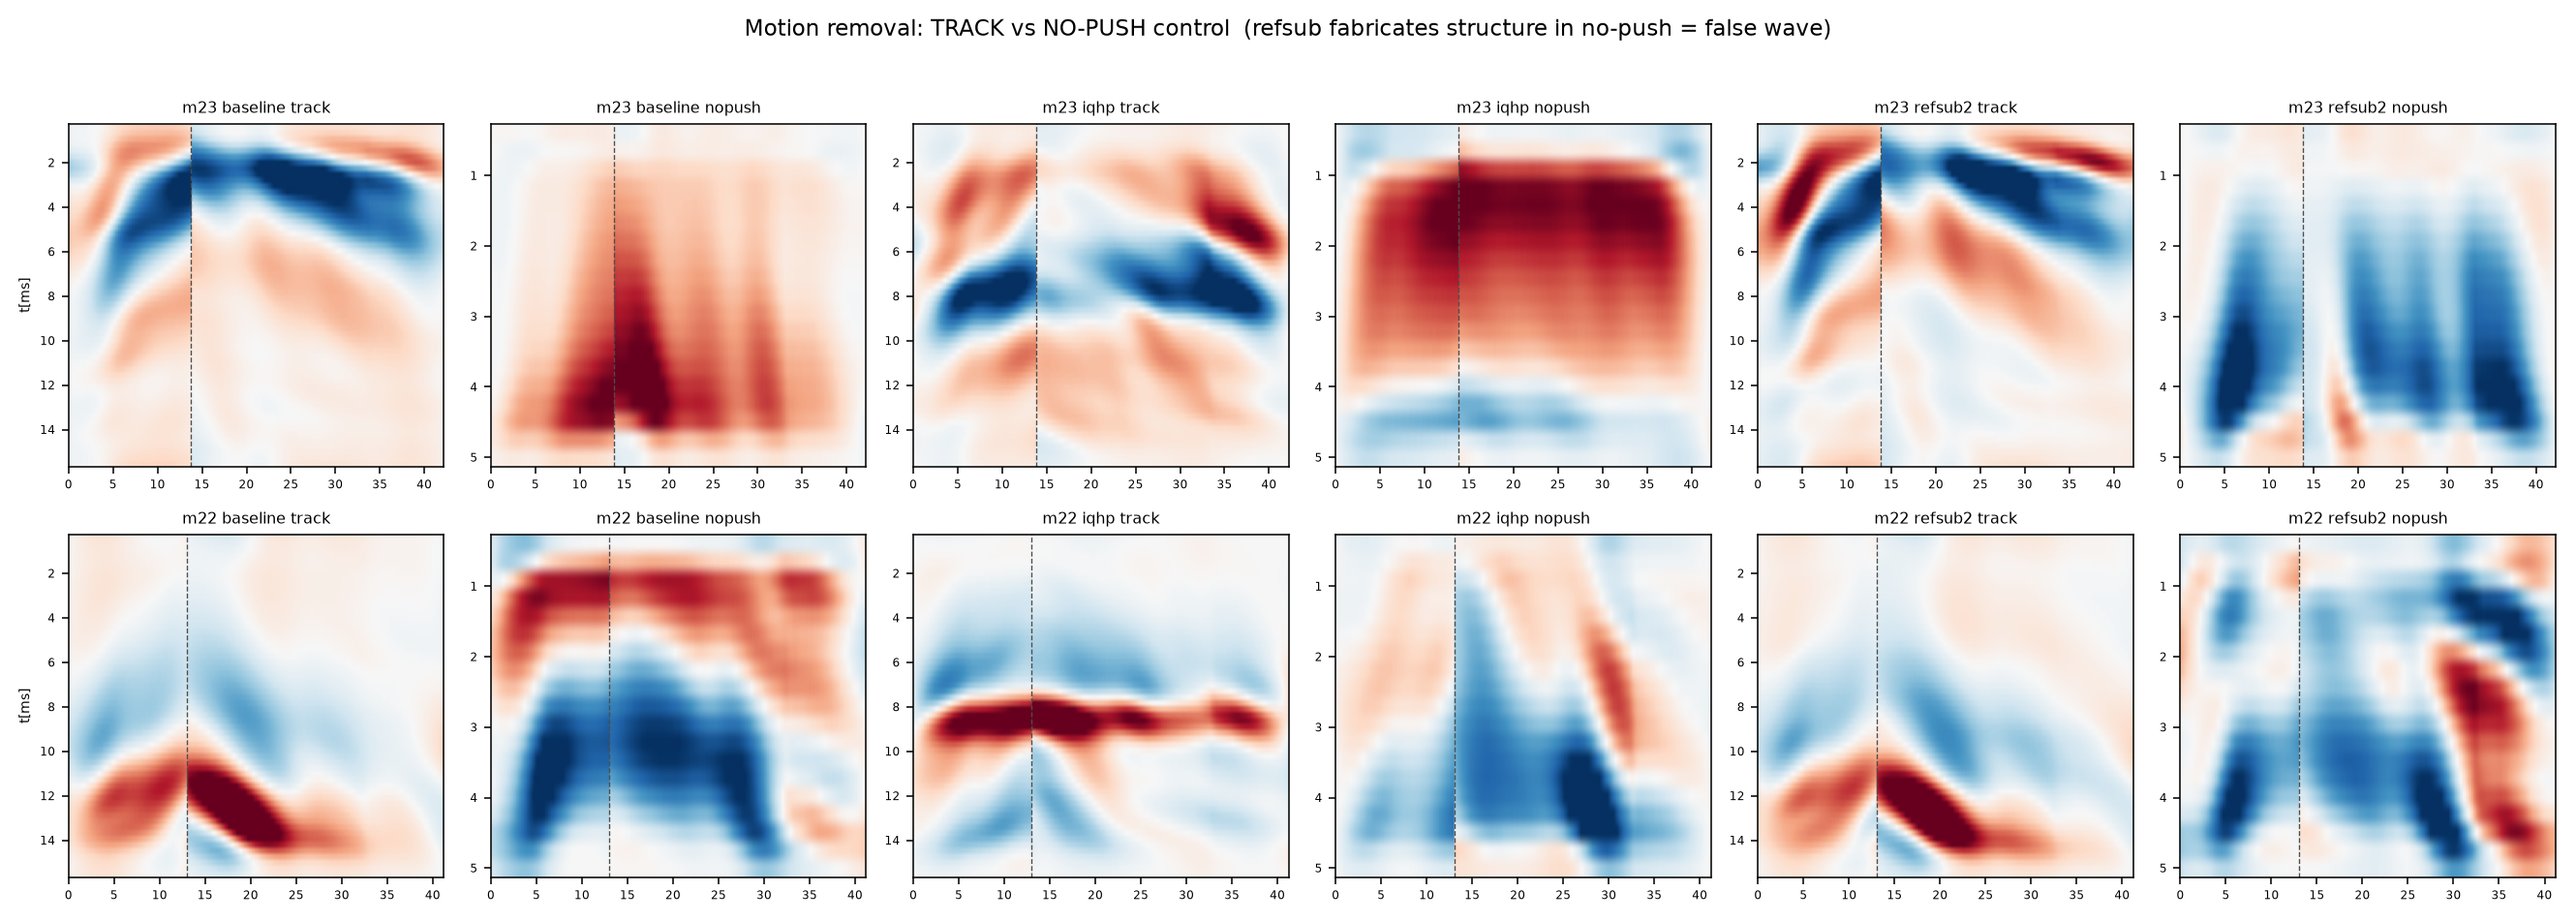
\includegraphics[width=\textwidth]{motion_removal_montage.png}
\caption{In-vivo cardiac-motion-removal harness. Validated with a split-reference no-push control, aggressive
filters (reference-subspace projection, SVD clutter) can \emph{fabricate} a false V from pure cardiac motion,
while honest removers that quiet the reference also remove the tracking ``signal'' --- because it is cardiac
motion. Processing cannot manufacture a wave that the acquisition did not capture.}
\label{fig:motionremoval}
\end{figure}

% ======================================================================
\section{Other suggestions and next steps}\label{sec:next}
% ======================================================================
In rough priority order, with the strongest lever first:

\begin{enumerate}
  \item \textbf{Re-acquire in vivo with a stronger, shallower push (highest priority).} Implement the
  \S\ref{sec:acq} recommendation: $\sim$61 push elements ($+48\%$ MI, within limits) and a
  $\sim$800\,\si{\micro s} pulse, focused on the nearest wall segment at the lowest achievable F-number, at
  the MI-limited voltage. This is the single biggest lever and directly targets the vibration-amplitude gap
  that Caenen's acquisition closes and ours does not.
  \item \textbf{Raise the tracking PRF} toward $\geq$5.6\,kHz with a shallow wall-only tracking window
  (watch for deep-echo range-wrap), and \textbf{ECG-gate / R-peak trigger} to place pushes at diastasis
  (the quiet cardiac phase) --- both narrow the motion floor the wave must exceed.
  \item \textbf{Then, and only then, apply the reference-trained motion filter.} With a wave actually above
  the motion floor, the optical-flow / bulk-motion compensation removers (validated by the no-push control)
  can clean up residual in-band wall motion. Until the wave is present, filtering only risks fabrication.
  \item \textbf{Confirmatory acquisition-parameter run:} a single 61-element $+$ long-pulse phantom
  acquisition (the exact recommended combination was interpolated, not measured), ideally with an absolute
  MI readout.
  \item \textbf{Passive SWE improvements:} promote a signed-Radon / slant-stack (wave-centre) speed estimator
  into the montage overlay, ECG-anchor the valve-closure window labelling (rather than timing arithmetic),
  and address the M-line-alignment-limited absolute-speed accuracy (\S\ref{sec:mline}) with a
  curvature/obliquity check.
  \item \textbf{Caenen stiffness read-out:} use the ECG timing to fit a systolic/diastolic piecewise SWS
  model rather than pooling per-push speeds, turning the recovered wave into a stiffness-vs-phase curve.
  \item \textbf{Optional processing extensions} noted but de-prioritised: true (non-reconstructed) RF
  beamforming for the fine-grid NCC, $f$--$k$ velocity-passband directional filtering, local phase-velocity
  imaging (dispersion-aware speed), and a smoothness/SNR-aware quality metric (the human's smoothness
  preference is not fully captured by \texttt{origin\_coherence}).
\end{enumerate}

% ======================================================================
\section{Conclusion}
% ======================================================================
The project delivers a working, modular cardiac-SWE pipeline; an interactive GUI that makes the large method
space tractable and exposes the \emph{no-push control} that keeps the analysis honest; and a validated,
SNR-adaptive recipe backed by a substantial blind human-scoring campaign. On controlled and real cardiac
data --- the phantom voltage sweep and the Caenen pig dataset --- it cleanly recovers the shear wave, with a
method family that is consistent across both. The honest limitation is our own in-vivo human acquisition,
which is \emph{acquisition-limited}: the push is too weak, too deep, and too loosely focused for the ARF wave
to rise above cardiac wall motion, and no amount of processing manufactures a wave that was not captured
(attempting to do so fabricates artifacts, as the no-push control proves). The path forward is therefore
concrete and evidence-backed --- a stronger, shallower, ECG-gated push --- after which the processing already
developed here should recover the wave, exactly as it does on the Caenen data.

% ======================================================================
\appendix
\section{Reference montages: displacement \& velocity, push \& pre-push, per dataset}\label{sec:appendix}
% ======================================================================
For completeness, this appendix shows every dataset through one common lens: for each push (or phantom
voltage) it displays \textbf{both} the displacement and the velocity space-time, and for each of those
\textbf{both} the post-push (tracking) window and the pre-push (no-push) reference window. All panels use
the same uniform recipe (Loupas / relative-to-reference / band-pass 120--700\,Hz / Gaussian smooth /
moving-mean / outward / 7 offsets), with the colour scale shared per column per quantity so push and
no-push are directly comparable. These are reference material; the main-text figures remain the curated,
recipe-appropriate views (e.g.\ the Caenen wave is read best in velocity with a narrower band,
Fig.~\ref{fig:caenen_pushnopush}).

The four rows of each block are, top to bottom: displacement PUSH, displacement no-push, velocity PUSH,
velocity no-push. Reading across the three datasets: on the \textbf{phantom} (Fig.~\ref{fig:app_phantom})
the push rows show the clean symmetric V degrading with voltage while the no-push rows stay comparatively
quiet (static medium); on \textbf{Caenen} (Figs.~\ref{fig:app_caenen_a}--\ref{fig:app_caenen_b}) the push
rows carry a coherent wave at essentially every push in both quantities; on the \textbf{in-vivo} data
(Fig.~\ref{fig:app_invivo}) the no-push rows are frequently as strong as (or stronger than) the push rows
--- the cardiac-motion signature --- except at the quiet-diastasis pushes. Note that the uniform
120--700\,Hz band is deliberately \emph{not} the Caenen-optimal band, so the Caenen displacement panels
here look weaker than the velocity panels, illustrating the SNR-dependent quantity choice of
\S\ref{sec:scoring} rather than any deficiency in the data.

\begin{figure}[p]
\centering
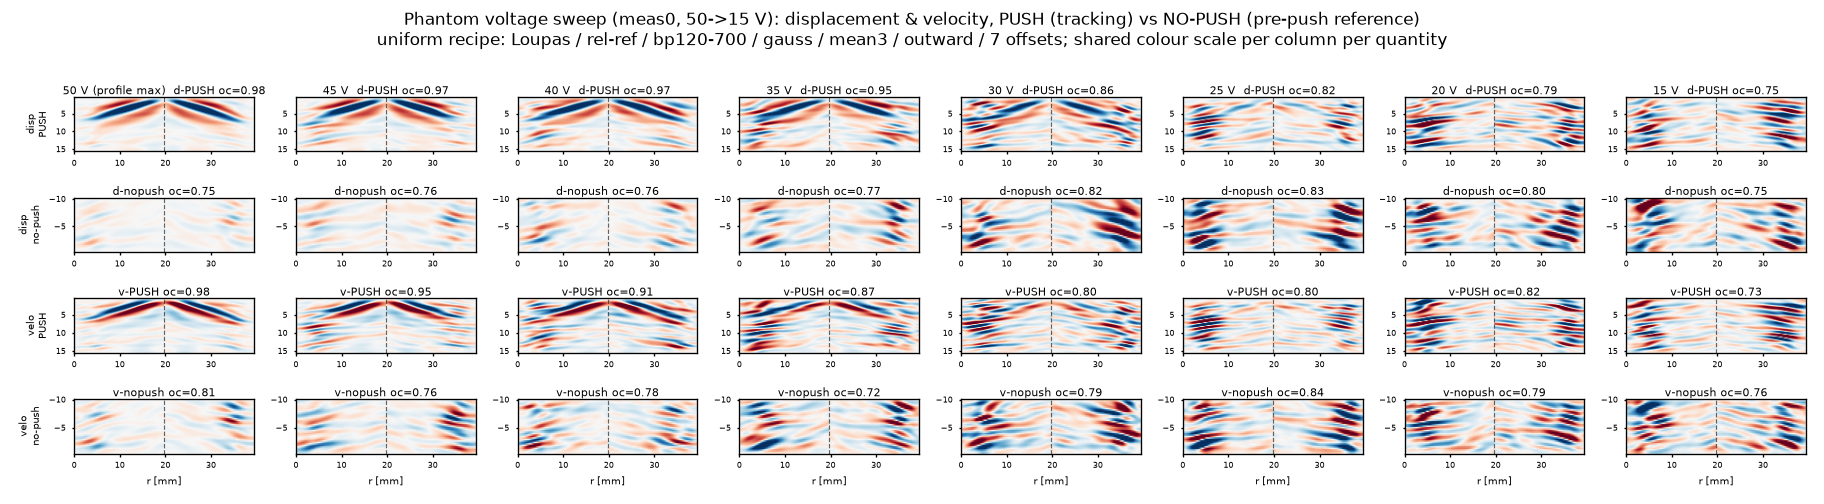
\includegraphics[width=\textwidth]{appendix_phantom.png}
\caption{\textbf{Phantom voltage sweep} (meas0, 50$\rightarrow$15\,V). Displacement and velocity, push and
no-push. The push rows show the symmetric outward V weakening monotonically with voltage; the no-push
(pre-push) rows stay comparatively quiet, as expected for a static medium.}
\label{fig:app_phantom}
\end{figure}

\begin{figure}[p]
\centering
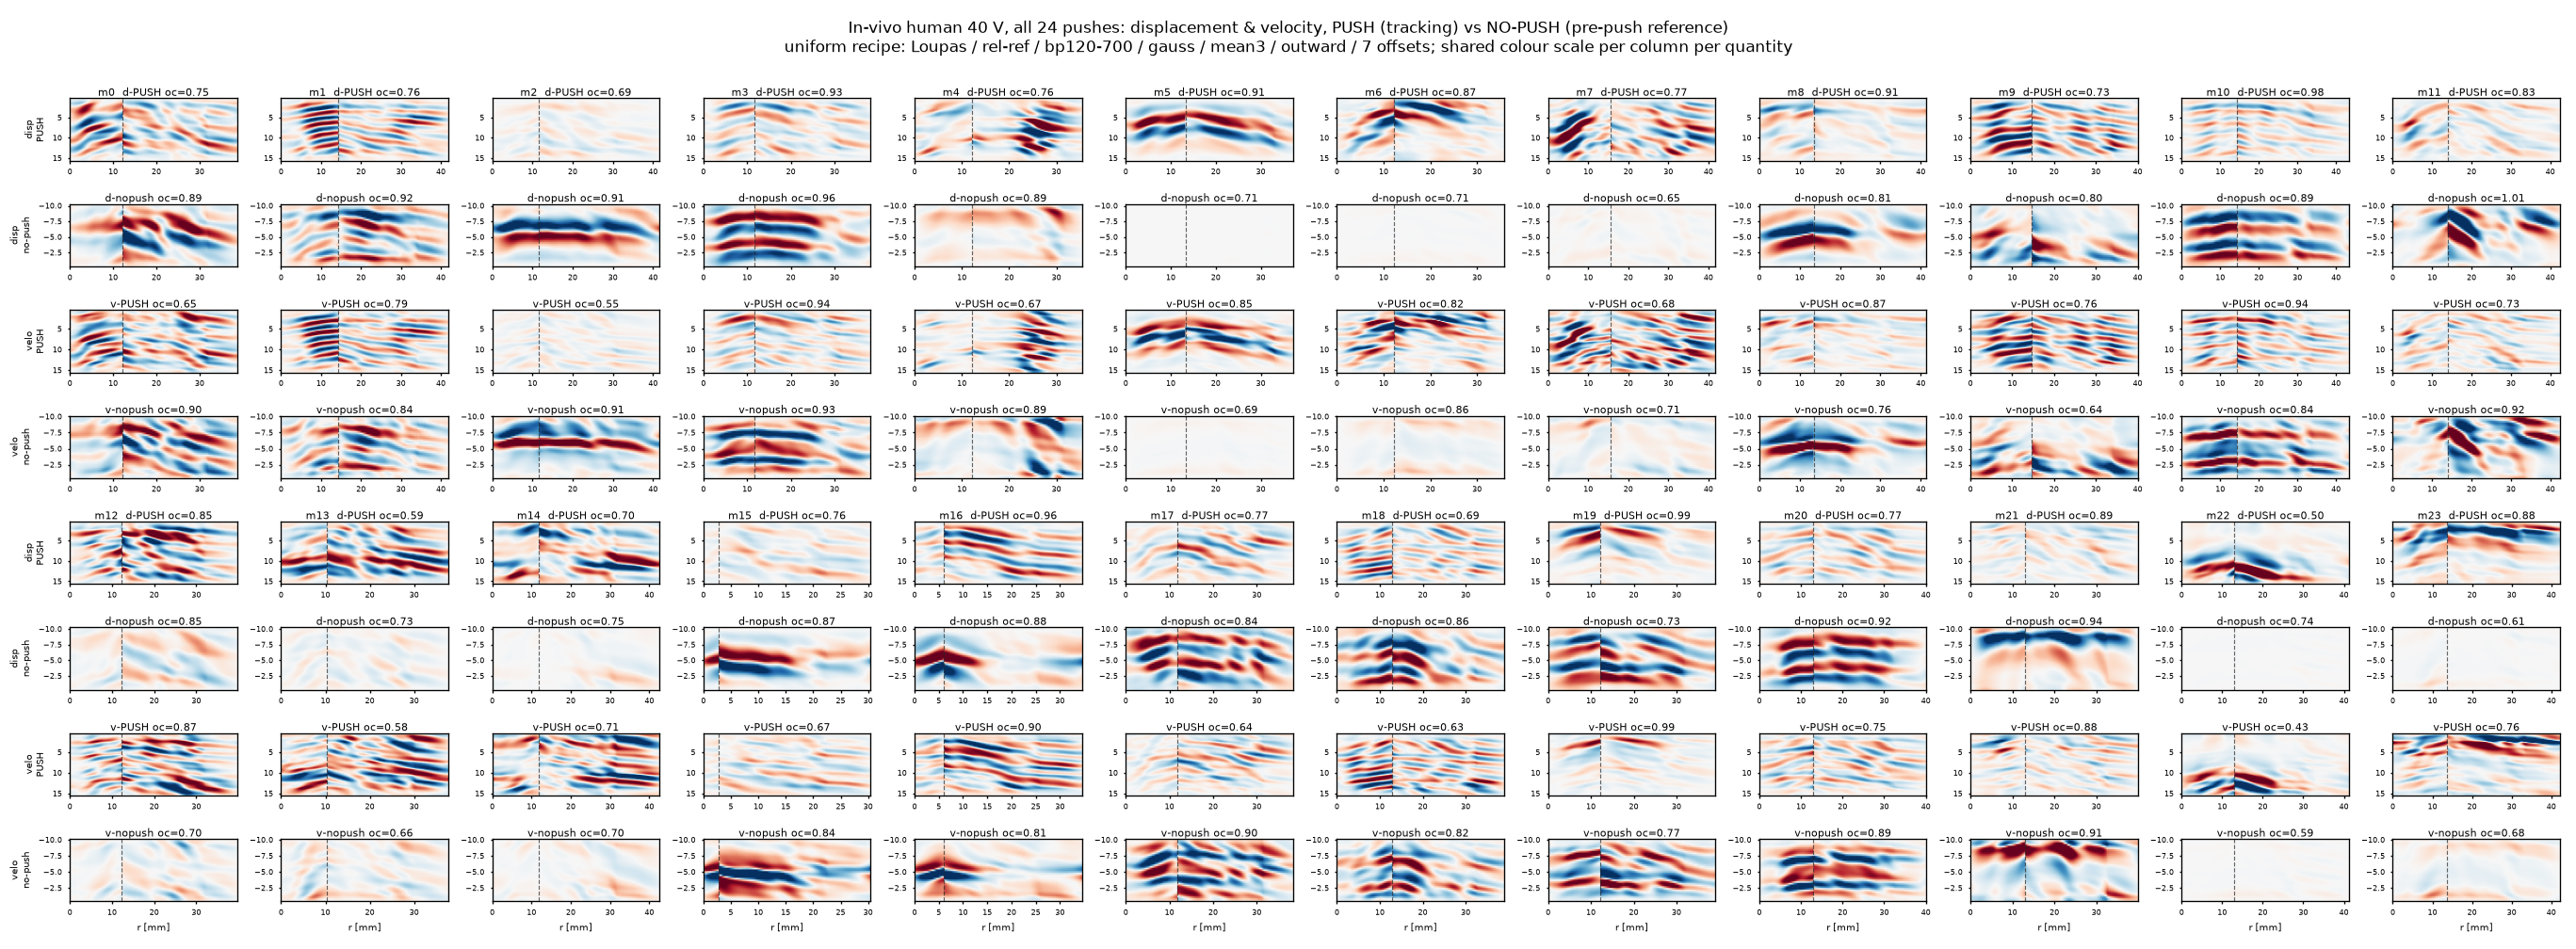
\includegraphics[width=\textwidth]{appendix_invivo40.png}
\caption{\textbf{In-vivo human 40\,V}, all 24 pushes. Displacement and velocity, push and no-push. In most
pushes the no-push (pre-push reference) rows are as strong as the push rows in both quantities --- the
cardiac-motion signature (\S\ref{sec:invivo}). The quiet-diastasis pushes (m5, m6, m22, m23) are the
exception, with quiet no-push rows.}
\label{fig:app_invivo}
\end{figure}

\begin{figure}[p]
\centering
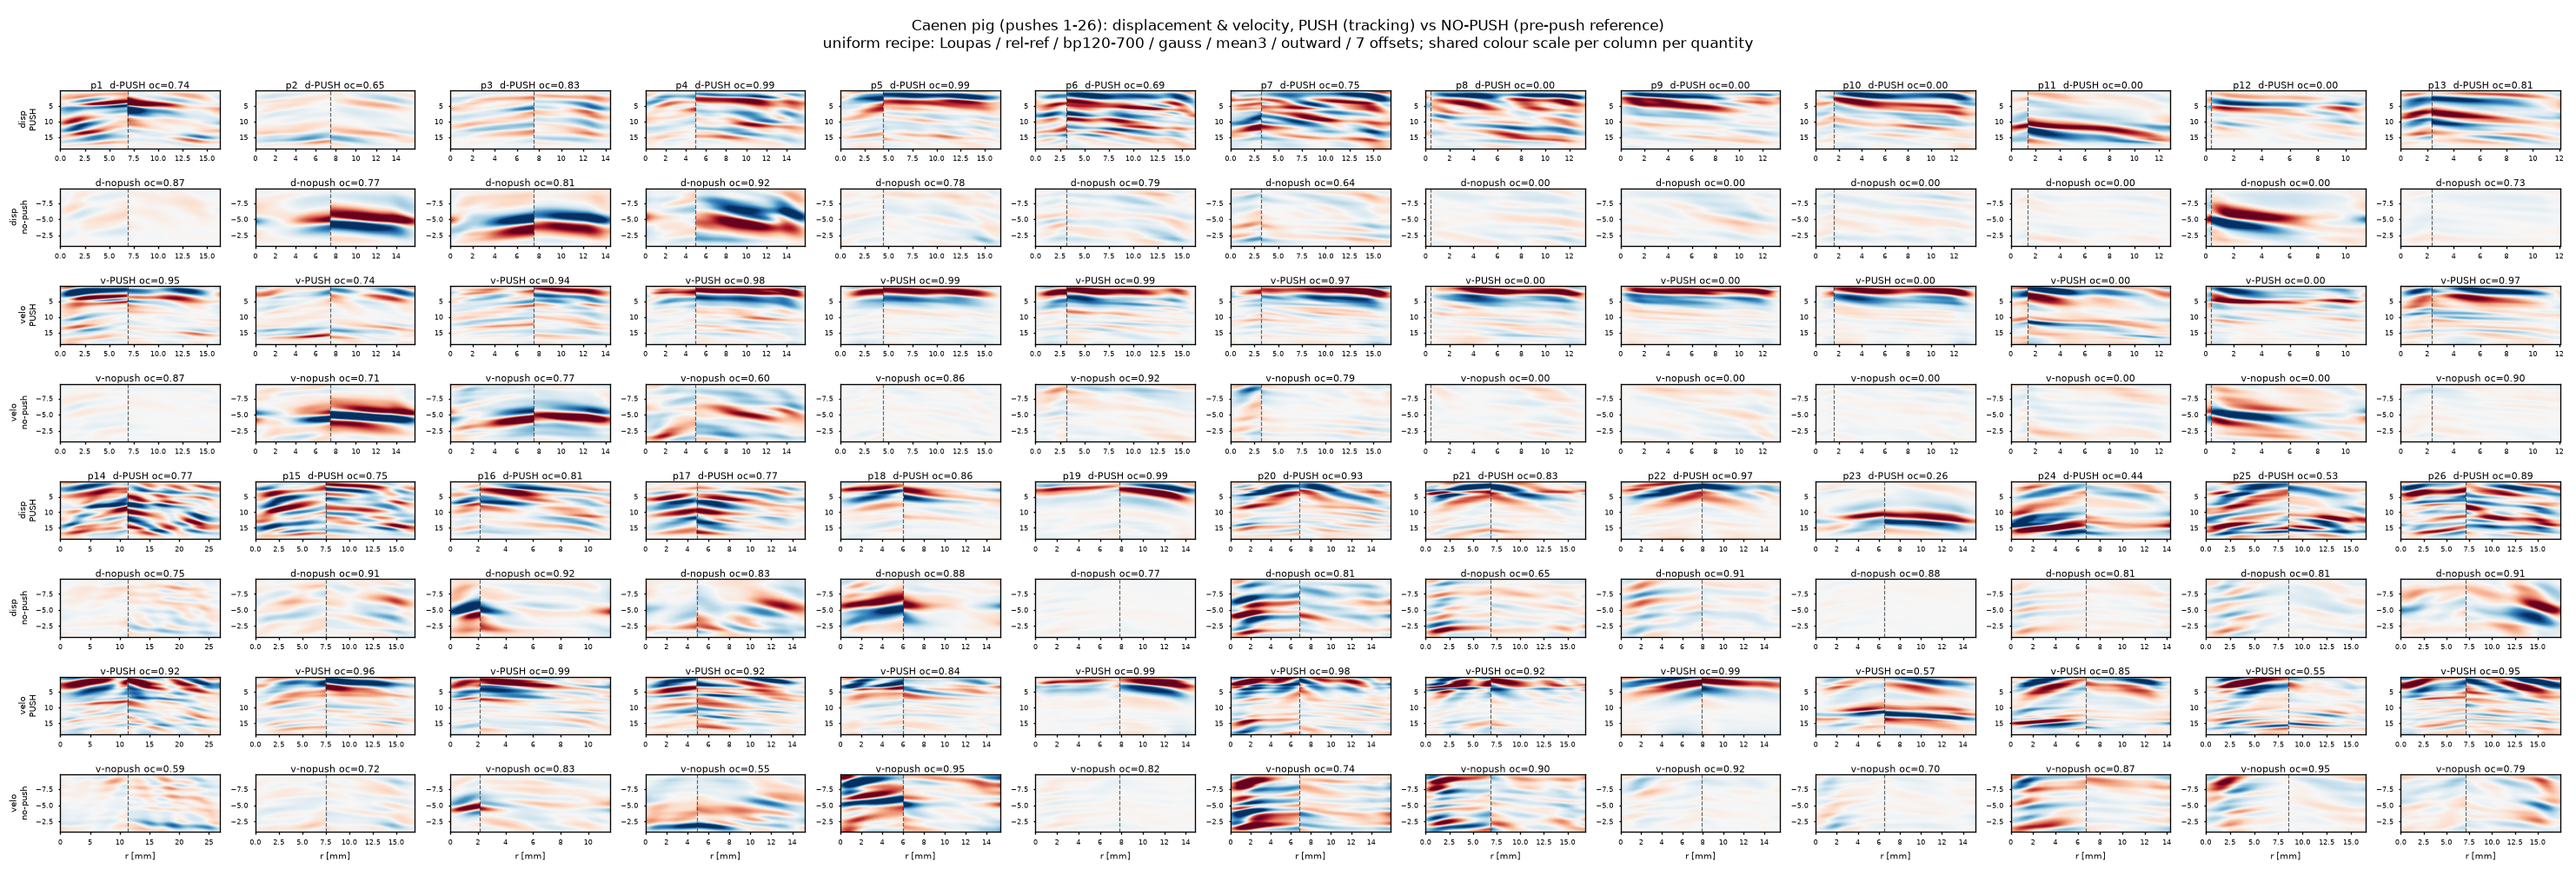
\includegraphics[width=\textwidth]{appendix_caenen_a.png}
\caption{\textbf{Caenen pig, pushes 1--26}. Displacement and velocity, push and no-push. A coherent wave
is present in the push rows at essentially every push (clearer in velocity, since the uniform 120--700\,Hz
band is not the Caenen-optimal narrow band).}
\label{fig:app_caenen_a}
\end{figure}

\begin{figure}[p]
\centering
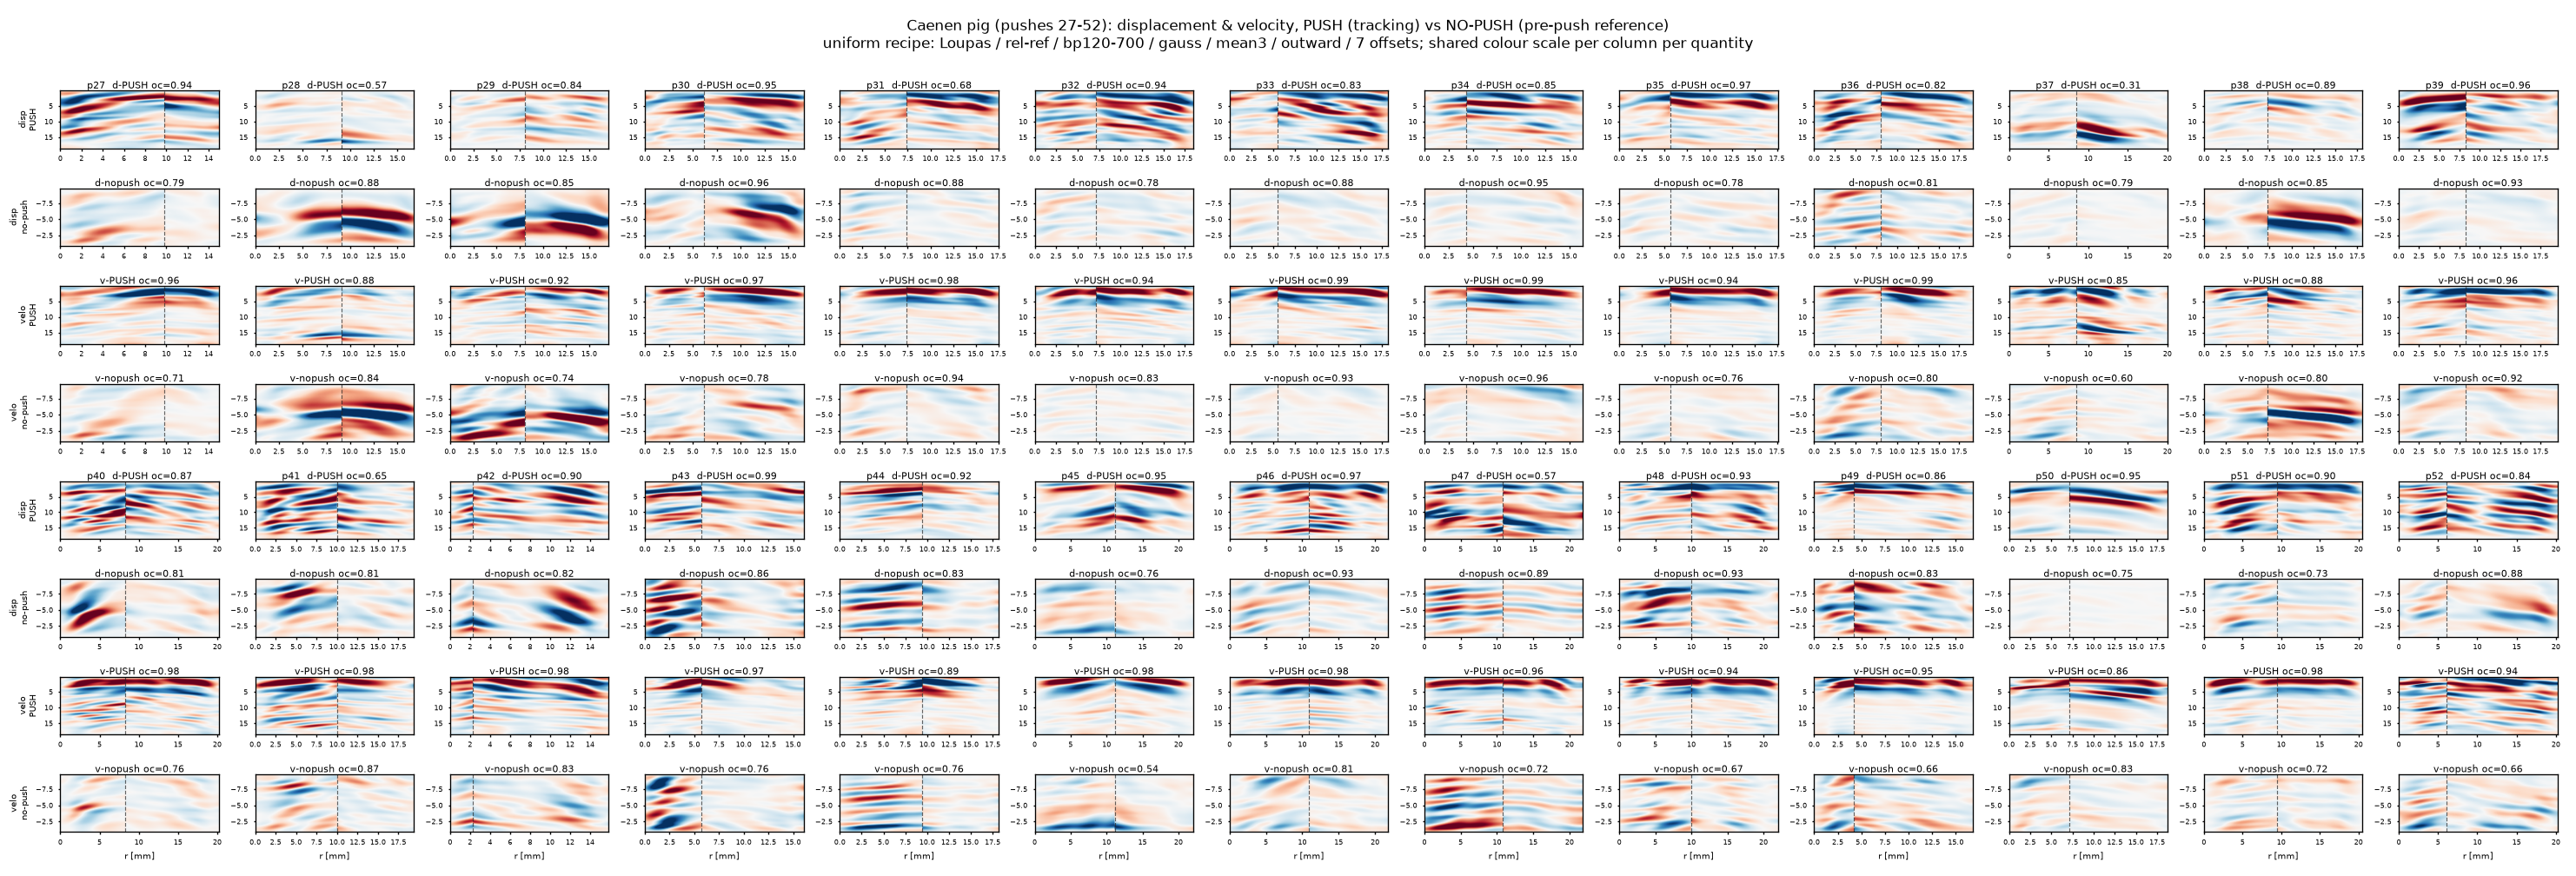
\includegraphics[width=\textwidth]{appendix_caenen_b.png}
\caption{\textbf{Caenen pig, pushes 27--52}. Displacement and velocity, push and no-push (continuation of
Fig.~\ref{fig:app_caenen_a}).}
\label{fig:app_caenen_b}
\end{figure}

% ======================================================================
\begin{thebibliography}{9}
\bibitem{strachinaru2020} M.~Strachinaru, J.~G.~Bosch, H.~J.~Vos, \emph{et al.},
``A direct comparison of natural and acoustic-radiation-force-induced cardiac mechanical waves,''
\emph{Sci.\ Rep.}, 2020.
\bibitem{vos2024} H.~J.~Vos, A.~I.~Petrescu, \emph{et al.},
``Ultrasound Shear Wave Elastography in Cardiology,'' \emph{JACC: Cardiovasc.\ Imaging}, 2024.
\bibitem{caenen2023} A.~Caenen, \emph{et al.},
``Continuous shear wave measurements for dynamic cardiac stiffness evaluation in pigs,''
\emph{Sci.\ Rep.}, 13:17660, 2023.
\bibitem{demene2015} C.~Demen\'e, \emph{et al.},
``Spatiotemporal Clutter Filtering of Ultrafast Ultrasound Data Highly Increases Doppler and fUltrasound
Sensitivity,'' \emph{IEEE Trans.\ Med.\ Imaging}, 2015.
\bibitem{pinton2006} G.~F.~Pinton, J.~J.~Dahl, G.~E.~Trahey,
``Rapid tracking of small displacements with ultrasound,'' \emph{IEEE Trans.\ UFFC}, 2006.
\bibitem{petrescu2022} A.~Petrescu, \emph{et al.},
``Comparing Myocardial Shear Wave Propagation Velocity Estimation Methods Based on Tissue Displacement,
Velocity and Acceleration Data,'' \emph{Ultrasound Med.\ Biol.}, 2022.
\bibitem{manduca2003} A.~Manduca, \emph{et al.},
``Spatio-temporal directional filtering for improved inversion of MR elastography images,''
\emph{Med.\ Image Anal.}, 2003.
\bibitem{mclaughlin2010} J.~McLaughlin, D.~Renzi, \emph{et al.},
``Robust estimation of time-of-flight shear wave speed using a Radon sum transformation,''
\emph{IEEE Trans.\ UFFC}, 2010.
\end{thebibliography}

\end{document}
